\documentclass[aspectratio=169]{beamer}

\usepackage[utf8]{inputenc}
\usepackage{graphicx}
\usepackage{xcolor}
\usepackage{lmodern}
\usepackage{amsmath,amssymb}
\usepackage{booktabs}
\usepackage{algorithm,algpseudocode}
\usepackage{appendixnumberbeamer}
\algrenewcommand{\algorithmicrequire}{\textbf{Input:}}
\algrenewcommand{\algorithmicensure}{\textbf{Output:}}

% Match the format of Results_Paper/main_combined_burgers_hgv2_v3.tex.
\definecolor{stanfordred}{HTML}{8C1515}
\definecolor{customlightgray}{rgb}{0.9,0.9,0.9}
\usetheme{Dresden}
\setbeamertemplate{headline}{}
\setbeamercolor{structure}{fg=stanfordred}
\setbeamercolor{title}{fg=stanfordred}
\setbeamercolor{frametitle}{bg=stanfordred,fg=white}
\setbeamercolor{itemize item}{fg=stanfordred}
\setbeamercolor{section in toc}{fg=stanfordred}
\setbeamercolor{section in head/foot}{bg=customlightgray,fg=stanfordred}
\setbeamerfont{section in head/foot}{size=\scriptsize}
\setbeamerfont{frametitle}{size=\small}
\setbeamertemplate{navigation symbols}{}
\setbeamertemplate{caption}[numbered]
\setbeamercolor{button}{bg=stanfordred,fg=white}
\newif\ifbmecswappendix
\newif\ifbmecswalgorithm
\renewcommand{\appendixname}{Appendix}
\setbeamertemplate{footline}{%
  \leavevmode%
  \hbox{%
    \ifbmecswalgorithm
      \begin{beamercolorbox}[wd=0.85\paperwidth,ht=2.5ex,dp=1ex,left]{normal text}%
        \hspace*{1em}{\fontsize{6.5}{7}\selectfont\textcolor{stanfordred}{Click a red line number for its explanation.}}%
      \end{beamercolorbox}%
    \else
      \hspace*{0.85\paperwidth}%
    \fi
    \begin{beamercolorbox}[wd=0.15\paperwidth,ht=2.5ex,dp=1ex,right]{date in head/foot}%
      \ifbmecswappendix A\fi\insertframenumber{} / \inserttotalframenumber%
    \end{beamercolorbox}%
  }%
}

\newcommand{\vect}[1]{\boldsymbol{#1}}
\newcommand{\matr}[1]{\boldsymbol{#1}}
\newcommand{\ECSWLinkedLineNumber}[1]{%
  \hyperlink{ecsw-line-#1}{\textcolor{stanfordred}{#1:}}%
}
\newcommand{\BMECSWLinkedLineNumber}[1]{%
  \hyperlink{bm-ecsw-line-#1}{\textcolor{stanfordred}{#1:}}%
}
\newcommand{\OnlineAlgorithmLineNumber}[1]{#1:}
\newcommand{\BackToClassicalAlgorithm}{%
  \par\vfill\hfill
  \hyperlink{ecsw-classical-algorithm}{\beamerreturnbutton{Back to algorithm}}%
}
\newcommand{\BackToBMAlgorithm}{%
  \par\vfill\hfill
  \hyperlink{ecsw-bm-algorithm}{\beamerreturnbutton{Back to BM algorithm}}%
}
\newcommand{\BackToOnlineComparison}{%
  \par\vfill\hfill
  \hyperlink{ecsw-online-comparison}{\beamerreturnbutton{Back to online comparison}}%
}
\title{By-mode \texorpdfstring{``ECSW''}{"ECSW"}}
\author{%
  Sebastian Ares de Parga\inst{1}\texorpdfstring{\\}{, }
  Sebastian Rodriguez Iturra\inst{3}\texorpdfstring{\\}{, }
  Charbel Farhat\inst{1,2}
}
\institute{%
  \inst{1} Department of Aeronautics and Astronautics\\
  \inst{2} Institute for Computational and Mathematical Engineering\\
  Stanford University, Stanford, CA 94305, USA\\[0.4em]
  \inst{3} PIMM (UMR 8006), Arts et M\'etiers, CNRS, Cnam, Paris, France
}
% Rodriguez Iturra affiliation: https://pimm.artsetmetiers.fr/en/directory
% PIMM partner institutions: https://recherche.cnam.fr/aap-recherche/pimm/laboratoire-procedes-et-ingenierie-en-mecanique-et-materiaux-pimm--658116.kjsp?RH=1643035801325&toPdf=true
\date{October 9, 2026}

% This independent presentation is developed one slide at a time.
% In this presentation N_c denotes training configurations, not clusters.
\begin{document}

\begin{frame}
  \titlepage
\end{frame}

\begin{frame}{Projected residuals: what BM-ECSW changes}
\small
\setlength{\abovedisplayskip}{1.5pt}
\setlength{\belowdisplayskip}{1.5pt}
\setlength{\abovedisplayshortskip}{1.5pt}
\setlength{\belowdisplayshortskip}{1.5pt}
At $\widetilde{\vect{u}}=\vect{u}_{\mathrm{ref}}+\matr{V}\vect{q}$,
$\vect{r}_e(\vect{q})$ contains the assembled HDM residual rows associated with entity $e$.\par
The local test-basis block is
\[
  \text{Galerkin:}\quad \matr{W}_e=\matr{V}_e,
  \qquad
  \text{LSPG:}\quad \matr{W}_e=\matr{J}_e\matr{V}_{e^+}.
\]
{\footnotesize $\matr{J}_e=\tfrac{\partial\vect{r}_e}{\partial\widetilde{\vect{u}}_{e^+}}$ is the local residual Jacobian;
$e^+$ contains all state entries needed to evaluate $\vect{r}_e$.\\
$\matr{V}_e$ and $\matr{V}_{e^+}$ contain the corresponding rows of the trial basis $\matr{V}$.}

\[
  \begin{aligned}
    \text{Full PROM:}\quad
    &\vect{r}_n(\vect{q})
      =\sum\nolimits_{e\in\mathcal E}\matr{W}_e^T\vect{r}_e,\\[4pt]
    \uncover<2->{\text{Classical ECSW:}\quad}
    &\uncover<2->{\widetilde{\vect{r}}_n^{\mathrm{ECSW}}(\vect{q})
      =\sum\nolimits_{e\in\widetilde{\mathcal E}}
        {\color{stanfordred}\xi_e}\matr{W}_e^T\vect{r}_e,}\\[4pt]
    \uncover<3->{\text{BM-ECSW:}\quad}
    &\uncover<3->{\widetilde{\vect{r}}_n^{\mathrm{BM}}(\vect{q})
      =\sum\nolimits_{e\in\widetilde{\mathcal E}}
        {\color{stanfordred}\matr{D}_e}\matr{W}_e^T\vect{r}_e.}
  \end{aligned}
\]
\[
  \uncover<3->{\matr{D}_e=\operatorname{diag}(\xi_{e,1},\ldots,\xi_{e,n}),
  \qquad \xi_e,\xi_{e,i}\geq0,
  \qquad \widetilde{\mathcal E}\subset\mathcal E.}
\]

\textbf{\uncover<2->{ECSW: one weight per entity.}\uncover<3->{ BM: one weight per entity and reduced component.}}

\smallskip
{\footnotesize\uncover<2->{The sampled mesh and weights are trained offline and fixed online.
All residual and test-basis blocks above are evaluated at the current $\vect{q}$.}}
\end{frame}

\begin{frame}{Classical ECSW: training problem}
\small
\setlength{\abovedisplayskip}{3pt}
\setlength{\belowdisplayskip}{3pt}
\setlength{\abovedisplayshortskip}{3pt}
\setlength{\belowdisplayshortskip}{3pt}
\textbf{Offline construction:} fit the full projected training target using nonnegative weights:
\[
  \min_{\vect{\xi}\geq\vect{0}}
  \frac12\left\|\matr{G}\vect{\xi}-\vect{b}\right\|_2^2,
  \qquad \vect{b}=\matr{G}\vect{1}.
\]

\textbf{Training data:} stack the local contributions over $N_c$ configurations:
\[
  \matr{G}=
  \begin{bmatrix}
    \vect{g}_1^{(1)} & \cdots & \vect{g}_{N_e}^{(1)}\\
    \vdots & \ddots & \vdots\\
    \vect{g}_1^{(N_c)} & \cdots & \vect{g}_{N_e}^{(N_c)}
  \end{bmatrix}
  \in\mathbb R^{nN_c\times N_e},
  \qquad
  \vect{g}_e^{(c)}=
  \left[\matr{W}_e^{(c)}\right]^T\vect{r}_e^{(c)}.
\]
{\footnotesize
  Each column represents one entity; each training configuration supplies $n$ rows.\\
  $n$: reduced modes; $N_e$: full-mesh entities.
}

\vspace{0.4em}
\textbf{Progressive sampling:} select entities and refit their weights by NNLS until the prescribed accuracy is attained:
\[
  \frac{\left\|\matr{G}\vect{\xi}-\vect{b}\right\|_2}
       {\left\|\vect{b}\right\|_2}\leq\tau,
  \qquad
  \widetilde{\mathcal E}=\{e:\xi_e>0\}.
\]
\end{frame}

% Full pseudocode from BM_ECSW_LSPG_notes.tex, Algorithm 1.
\bmecswalgorithmtrue
\begin{frame}[t]{Classical ECSW: mesh sampling by NNLS}
\fontsize{7.5}{8.2}\selectfont
\let\alglinenumber\ECSWLinkedLineNumber
\begin{algorithmic}[1]
  \setlength{\itemsep}{0pt}
  \Require \hypertarget{ecsw-classical-algorithm}{%
    $\matr{G}=[\vect{g}_e]$, $\vect{b}\neq\vect{0}$, tolerance $\tau\in(0,1)$}
  \Ensure Weights $\vect{\xi}\geq\vect{0}$ and reduced mesh $\widetilde{\mathcal E}$
  \State $k\gets0$
  \State $\mathcal I^0\gets\varnothing$; $\mathcal Z^0\gets\mathcal E$
  \State $\vect{\xi}^{\,0}\gets\vect{0}$
  \State $\vect{h}^{\,0}\gets\vect{b}$
  \While{$\|\vect{h}^{\,k}\|_2>\tau\|\vect{b}\|_2$}
    \State Compute the correlations: $\vect{\mu}^{\,k}\gets\matr{G}^T\vect{h}^{\,k}$
    \State Select the most correlated entity: $e^k\gets\arg\max_{e\in\mathcal Z^k}\mu_e^k$
    \State Add the candidate: $\mathcal I^{k+1}\gets\mathcal I^k\cup\{e^k\}$
    \State Update the unselected set: $\mathcal Z^{k+1}\gets\mathcal E\setminus\mathcal I^{k+1}$
    \State Refit the weights of all selected entities by NNLS:
    \Statex \hspace{\algorithmicindent}$\displaystyle
      \vect{\xi}^{\,k+1}_{\mathcal I^{k+1}}\in
      \underset{\vect{z}\geq\vect{0}}{\arg\min}
      \frac12\|\matr{G}_{\mathcal I^{k+1}}\vect{z}-\vect{b}\|_2^2$
    \State Set unselected weights to zero: $\vect{\xi}^{\,k+1}_{\mathcal Z^{k+1}}\gets\vect{0}$
    \State Recompute the full fitting residual: $\vect{h}^{\,k+1}\gets\vect{b}-\matr{G}\vect{\xi}^{\,k+1}$
    \State $k\gets k+1$
  \EndWhile
  \State $\widetilde{\mathcal E}\gets\{e\in\mathcal E:\xi_e^{\,k}>0\}$
  \State \Return $\vect{\xi}^{\,k}$ and $\widetilde{\mathcal E}$
\end{algorithmic}
\end{frame}
\bmecswalgorithmfalse

\begin{frame}{BM-ECSW: modal weight training}
\small
\setlength{\abovedisplayskip}{3pt}
\setlength{\belowdisplayskip}{3pt}
\setlength{\abovedisplayshortskip}{3pt}
\setlength{\belowdisplayshortskip}{3pt}
\textbf{Offline construction:} fit the projected contributions with one weight vector per mode:
\[
  \min_{\vect{\xi}^{[i]}\geq\vect{0}}
  \frac12\|\matr{G}^{[i]}\vect{\xi}^{[i]}-\vect{b}^{[i]}\|_2^2,
  \qquad
  \vect{\xi}^{[i]}=[\xi_{1,i},\ldots,\xi_{N_e,i}]^T.
\]

\textbf{Same data, grouped by mode:} collect the rows of $\matr{G}$ associated with reduced equation $i$, one per training configuration:
\[
  \matr{G}^{[i]}=
  \begin{bmatrix}
    g_{1,i}^{(1)} & \cdots & g_{N_e,i}^{(1)}\\
    \vdots & \ddots & \vdots\\
    g_{1,i}^{(N_c)} & \cdots & g_{N_e,i}^{(N_c)}
  \end{bmatrix}
  \in\mathbb R^{N_c\times N_e},
  \qquad
  \begin{gathered}
    g_{e,i}^{(c)}=[\matr{W}_e^{(c)}(:,i)]^T\vect{r}_e^{(c)},\\[3pt]
    \vect{b}^{[i]}=\matr{G}^{[i]}\vect{1}.
  \end{gathered}
\]
{\footnotesize $e$: entity; $i$: reduced equation; $c$: training configuration.}\par
\vspace{0.2em}
\textbf{One shared mesh, one accuracy target:} combine the modal fitting errors:
\[
  \vect{h}^{[i]}=\vect{b}^{[i]}-\matr{G}^{[i]}\vect{\xi}^{[i]},
  \qquad
  \eta^2=\frac{\sum_i\|\vect{h}^{[i]}\|_2^2}
                {\sum_i\|\vect{b}^{[i]}\|_2^2}\leq\tau^2.
\]
{\footnotesize Entities are selected jointly; on the selected set, each mode's weights are refitted independently.}
\end{frame}

% Full pseudocode from BM_ECSW_LSPG_notes.tex, Algorithm 3.
\bmecswalgorithmtrue
\begin{frame}[t]{BM-ECSW: mesh sampling by modal NNLS}
\fontsize{7}{7.4}\selectfont
\let\alglinenumber\BMECSWLinkedLineNumber
\begin{algorithmic}[1]
  \setlength{\itemsep}{-0.6pt}
  \Require \hypertarget{ecsw-bm-algorithm}{%
    $\matr{G}^{[i]}=[\vect{g}_e^{[i]}]$, $\vect{b}^{[i]}$ with $\sum_i\|\vect{b}^{[i]}\|_2^2>0$, tolerance $\tau\in(0,1)$}
  \Ensure Modal weights $\vect{\xi}^{[i]}\geq\vect{0}$ and reduced mesh $\widetilde{\mathcal E}$
  \State $k\gets0$; $\mathcal I^0\gets\varnothing$; $\mathcal Z^0\gets\mathcal E$
  \State $\vect{\xi}^{[i],0}\gets\vect{0}$; $\vect{h}^{[i],0}\gets\vect{b}^{[i]}$ for every $i$
  \While{$\sum_i\|\vect{h}^{[i],k}\|_2^2>\tau^2\sum_i\|\vect{b}^{[i]}\|_2^2$}
    \State Sum the modal correlations: $\textstyle\vect{\mu}^{\,k}\gets\sum_{i=1}^n[\matr{G}^{[i]}]^T\vect{h}^{[i],k}$
    \State Select the most correlated entity: $e^k\gets\arg\max_{e\in\mathcal Z^k}\mu_e^k$
    \State Add the candidate: $\mathcal I^{k+1}\gets\mathcal I^k\cup\{e^k\}$
    \State Update the unselected set: $\mathcal Z^{k+1}\gets\mathcal E\setminus\mathcal I^{k+1}$
    \For{$i=1,\ldots,n$}
      \State Refit the selected weights of mode $i$ by NNLS:
      \Statex \hspace{\dimexpr\algorithmicindent+\algorithmicindent\relax}$\displaystyle
        \vect{\xi}^{[i],k+1}_{\mathcal I^{k+1}}\in
        \underset{\vect{z}\geq\vect{0}}{\arg\min}
        \frac12\|\matr{G}^{[i]}_{\mathcal I^{k+1}}\vect{z}-\vect{b}^{[i]}\|_2^2$
      \State Set unselected weights to zero: $\vect{\xi}^{[i],k+1}_{\mathcal Z^{k+1}}\gets\vect{0}$
      \State Recompute the fitting residual: $\vect{h}^{[i],k+1}\gets\vect{b}^{[i]}-\matr{G}^{[i]}\vect{\xi}^{[i],k+1}$
    \EndFor
    \State $k\gets k+1$
  \EndWhile
  \State $\textstyle\widetilde{\mathcal E}\gets\bigcup_{i=1}^n\{e\in\mathcal E:\xi_{e,i}^{\,k}>0\}$
  \State \Return $\{\vect{\xi}^{[i],k}\}_{i=1}^n$ and $\widetilde{\mathcal E}$
\end{algorithmic}
\end{frame}
\bmecswalgorithmfalse

\begin{frame}{LSPG online solution: classical ECSW and BM-ECSW}
\small
\setlength{\abovedisplayskip}{4pt}
\setlength{\belowdisplayskip}{4pt}
\setlength{\abovedisplayshortskip}{4pt}
\setlength{\belowdisplayshortskip}{4pt}
\hypertarget{ecsw-online-comparison}{\textbf{Online target:}}
solve $\widetilde{\vect{r}}_n(\vect{q})=\vect{0}$ at each time step,
with the trained mesh and weights fixed.
\vspace{0.2em}

\textbf{At iteration $k$:}
$\vect{r}_e^k=\vect{r}_e(\vect{q}^k)$ and
$\matr{W}_e^k=\tfrac{\partial\vect{r}_e}{\partial\vect{q}}(\vect{q}^k)$.
\vspace{0.5em}

\setlength{\fboxsep}{4pt}
\setlength{\fboxrule}{0.4pt}
\begin{columns}[T,onlytextwidth]
  \begin{column}{0.49\textwidth}
    \fcolorbox{black!25}{black!2}{%
      \begin{minipage}[t][4.8cm][t]{\dimexpr\linewidth-2\fboxsep-2\fboxrule\relax}
        \vspace{0pt}

    \textbf{HPROM (ECSW)}\par\vspace{0.15em}\footnotesize

    \begin{minipage}[t][1.30cm][t]{\linewidth}
      \vspace{0pt}
      \textbf{Sampled projected residual:}
    \[
      \widetilde{\vect{r}}_n^{\mathrm{ECSW},k}
      =\sum\nolimits_{e\in\widetilde{\mathcal E}}
        {\color{stanfordred}\xi_e}[\matr{W}_e^k]^T\vect{r}_e^k.
    \]
    \end{minipage}\par
    \begin{minipage}[t][1.30cm][t]{\linewidth}
      \vspace{0pt}
      \textbf{Gauss--Newton Jacobian approximation:}
    \[
      \widehat{\matr{J}}_n^{\mathrm{ECSW},k}
      =\sum\nolimits_{e\in\widetilde{\mathcal E}}
        {\color{stanfordred}\xi_e}[\matr{W}_e^k]^T\matr{W}_e^k.
    \]
    \end{minipage}\par
    \begin{minipage}[t][1.10cm][t]{\linewidth}
      \vspace{0pt}
      \textbf{Coupled correction:}
    \[
      \widehat{\matr{J}}_n^{\mathrm{ECSW},k}\Delta\vect{q}^k
      =-\widetilde{\vect{r}}_n^{\mathrm{ECSW},k}.
    \]
    \end{minipage}\par
    \vfill\hyperlink{ecsw-online-classical-algorithm}{\beamerbutton{Classical online algorithm}}

      \end{minipage}%
    }
  \end{column}
  \begin{column}{0.49\textwidth}
    \fcolorbox{black!25}{black!2}{%
      \begin{minipage}[t][4.8cm][t]{\dimexpr\linewidth-2\fboxsep-2\fboxrule\relax}
        \vspace{0pt}

    \textbf{HPROM (BM-ECSW)}\par\vspace{0.15em}\footnotesize

    \begin{minipage}[t][1.30cm][t]{\linewidth}
      \vspace{0pt}
      \textbf{Sampled projected residual:}
    \[
      \widetilde{\vect{r}}_n^{\mathrm{BM},k}
      =\sum\nolimits_{e\in\widetilde{\mathcal E}}
        {\color{stanfordred}\matr{D}_e}[\matr{W}_e^k]^T\vect{r}_e^k.
    \]
    \end{minipage}\par
    \begin{minipage}[t][1.30cm][t]{\linewidth}
      \vspace{0pt}
      \textbf{Gauss--Newton-type Jacobian approximation:}
    \[
      \widehat{\matr{J}}_n^{\mathrm{BM},k}
      =\sum\nolimits_{e\in\widetilde{\mathcal E}}
        {\color{stanfordred}\matr{D}_e}[\matr{W}_e^k]^T\matr{W}_e^k.
    \]
    \end{minipage}\par
    \begin{minipage}[t][1.10cm][t]{\linewidth}
      \vspace{0pt}
      \textbf{Coupled correction:}
    \[
      \widehat{\matr{J}}_n^{\mathrm{BM},k}\Delta\vect{q}^k
      =-\widetilde{\vect{r}}_n^{\mathrm{BM},k}.
    \]
    \end{minipage}\par
    \vfill\hyperlink{ecsw-online-bm-algorithm}{\beamerbutton{BM online algorithm}}

      \end{minipage}%
    }
  \end{column}
\end{columns}

\vspace{0.45em}
\textbf{Update all coordinates together:}
$\vect{q}^{k+1}=\vect{q}^k+\Delta\vect{q}^k$.
\vspace{0.2em}

{\footnotesize\textbf{Correction matrices:} classical, symmetric positive semidefinite;
BM, possibly nonsymmetric.}
\end{frame}

\begin{frame}[t]{What BM-ECSW gains in Burgers}
\setlength{\parskip}{0pt}
{\scriptsize 2D parametric inviscid Burgers; same ROB and training data
($N_e=62\,500$, $n=96$, $N_c=225$, $\tau=10^{-5}$).}\par
\footnotesize

\vspace{0.45em}
\textbf{Offline}\par\vspace{0.2em}
\begingroup
\centering
\footnotesize\rmfamily
\setlength{\tabcolsep}{3pt}
\renewcommand{\arraystretch}{1.08}
\resizebox{0.75\textwidth}{!}{%
\begin{tabular}{@{}lrrrrr@{}}
\toprule
Computational model & $n$ & $n_e$ & $n_e^+$ & $\eta$ & \shortstack{Offline training\\time (min)}\\
\midrule
HPROM (ECSW) & 96 & 2\,492 & 5\,914 & $9.795\times10^{-6}$ & 112.56\\
HPROM (BM-ECSW) & 96 & 300 & 868 & $8.359\times10^{-6}$ & 4.10\\
\bottomrule
\end{tabular}
%
}\par
\endgroup

\begin{uncoverenv}<2->
\vspace{0.45em}
\textbf{Online}\par\vspace{0.2em}
\begingroup
\centering
\footnotesize\rmfamily
\setlength{\tabcolsep}{3pt}
\renewcommand{\arraystretch}{1.08}
\resizebox{0.98\textwidth}{!}{%
\begin{tabular}{@{}lrrrrrr@{}}
\toprule
Computational model & \shortstack{$n$\\($N$ for HDM)} & \shortstack{$n_e$\\($N_e$ for HDM)} & $n_e^+$ & $\mathbb{RE}_{2,\vect{u}}^{\max}$ (\%) & \shortstack{Wall-clock time\\(min)} & \shortstack{Speedup\\factor}\\
\midrule
HDM & 125\,000 & 62\,500 & 62\,500 & -- & 5.404 & --\\
HPROM (ECSW) & 96 & 2\,492 & 5\,914 & 1.096 & 0.311 & 17.39\\
HPROM (BM-ECSW) & 96 & 300 & 868 & 1.102 & 0.020 & 267.93\\
\bottomrule
\end{tabular}
}\par
\endgroup
\end{uncoverenv}

\vspace{0.45em}
{\scriptsize\uncover<2->{\textbf{8.31$\times$ fewer cells; 27.48$\times$ faster training;
15.4$\times$ lower online time; comparable accuracy.}}}\par

\vspace{0.25em}
{\fontsize{7}{8}\selectfont
$n_e^+$: augmented-mesh cells. Offline excludes HDM generation and POD; speedups use unrounded times.
}\par
\vspace{0.15em}
\begin{uncoverenv}<3->
{\fontsize{8.5}{10}\selectfont\color{stanfordred}
\textbf{With $N_c=90$: 145 cells, but $4\,411.533\%$ maximum trajectory error.}
}
\end{uncoverenv}
\end{frame}

\begin{frame}{One common scalar function: the required property}
\fontsize{9.5}{11}\selectfont
\setlength{\parskip}{0pt}
\setlength{\abovedisplayskip}{0pt}
\setlength{\belowdisplayskip}{0pt}
\setlength{\abovedisplayshortskip}{0pt}
\setlength{\belowdisplayshortskip}{0pt}
\textbf{Goal: preserve $\vect{F}=\nabla_{\vect{q}}\Phi$ after weighting, so that LSPG retains one common error objective
and structural dynamics retains one common potential.}\par
$\vect{F}$: LSPG projected residual; reduced structural internal vector obtained by Galerkin projection.\\
{\footnotesize Smooth local scalar for entity $e$:
LSPG: $\phi_e=\tfrac12\|\vect{r}_e(\vect{q})\|_2^2$;
structures: $\phi_e=\mathcal V_{e,r}^{\mathrm{int}}(\vect{q})$.}\par
\[
  \vect{F}(\vect{q})
  =\sum\nolimits_{e\in\mathcal E}\nabla_{\vect{q}}\phi_e(\vect{q}).
\]

\uncover<2->{\textbf{Now we can connect these local functions to one common scalar function.}}
\[
  \uncover<2->{\Phi(\vect{q})=\sum\nolimits_{e\in\mathcal E}\phi_e(\vect{q}),
  \qquad
  \boxed{\vect{F}=\nabla_{\vect{q}}\Phi},
  \qquad
  F_i=\frac{\partial\Phi}{\partial q_i},
  \qquad i=1,\ldots,n.}
\]
\uncover<3->{\textbf{The question is whether the weighted vector is still the gradient of one common scalar function.}}\par
\uncover<3->{If $\vect{F}=\nabla_{\vect{q}}\Phi$, differentiating $F_i$ in $q_j$ differentiates $\Phi$ first in $q_i$, then in $q_j$.}\par
\uncover<3->{Differentiating $F_j$ in $q_i$ reverses the order. Continuous second derivatives give the same result:}
\[
  \uncover<3->{\frac{\partial F_i}{\partial q_j}
  =\frac{\partial^2\Phi}{\partial q_j\partial q_i}
  =\frac{\partial^2\Phi}{\partial q_i\partial q_j}
  =\frac{\partial F_j}{\partial q_i}.}
\]

\vspace{-0.7em}
\uncover<4->{\textbf{Preserving this connection allows us to retain the following classical properties:}}\par
\setlength{\topsep}{0pt}
\begin{itemize}
  \setlength{\itemsep}{0pt}
  \item<4-> \textbf{LSPG:} the classical Gauss--Newton correction minimizes one common quadratic error.
  \item<4-> \textbf{Structural dynamics:} one common potential defines the Lagrangian and conserved energy.
\end{itemize}
{\fontsize{8}{9}\selectfont \uncover<4->{Structures: same reduced kinetic energy, continuous time. BM may still converge without this structure.}}
\end{frame}


\begin{frame}{Scalar weights preserve it; modal weights do not guarantee it}
\fontsize{9.5}{11}\selectfont
\hypertarget<4>{bmecsw-weighting-comparison}{}
\setlength{\parskip}{0pt}
\setlength{\abovedisplayskip}{1pt}
\setlength{\belowdisplayskip}{1pt}
\setlength{\abovedisplayshortskip}{1pt}
\setlength{\belowdisplayshortskip}{1pt}
{\footnotesize The sampled mesh $\widetilde{\mathcal E}$ and the trained weights are fixed.}\par
\textbf{First, apply classical ECSW: one weight per entity, shared by all components.}
\[
  \vect{F}_{\mathrm{ECSW}}
  =\sum\nolimits_{e\in\widetilde{\mathcal E}}\xi_e\nabla_{\vect{q}}\phi_e.
\]
\uncover<2->{\textbf{The same weight keeps each pair equal and preserves one common scalar function.}}
\[
  \uncover<2->{
  \frac{\partial F_{\mathrm{ECSW},i}}{\partial q_j}
  -\frac{\partial F_{\mathrm{ECSW},j}}{\partial q_i}
  =\sum\nolimits_{e\in\widetilde{\mathcal E}}\xi_e
  \left[\frac{\partial^2\phi_e}{\partial q_j\partial q_i}
       -\frac{\partial^2\phi_e}{\partial q_i\partial q_j}\right]
  =0.}
\]
\[
  \uncover<2->{\Phi_{\mathrm{ECSW}}=\sum\nolimits_{e\in\widetilde{\mathcal E}}\xi_e\phi_e,
  \qquad
  \nabla_{\vect{q}}\Phi_{\mathrm{ECSW}}
  =\sum\nolimits_{e\in\widetilde{\mathcal E}}\xi_e\nabla_{\vect{q}}\phi_e
  =\vect{F}_{\mathrm{ECSW}}.}
\]
\uncover<3->{\textbf{Now apply BM-ECSW: components of one entity can receive different weights.}}
\[
  \uncover<3->{\vect{F}_{\mathrm{BM}}
  =\sum\nolimits_{e\in\widetilde{\mathcal E}}\matr{D}_e\nabla_{\vect{q}}\phi_e,
  \qquad
  F_{\mathrm{BM},i}
  =\sum\nolimits_{e\in\widetilde{\mathcal E}}\xi_{e,i}\frac{\partial\phi_e}{\partial q_i}.}
\]
\uncover<4->{\textbf{The local derivatives agree, but they can be multiplied by different weights.}}
\[
  \uncover<4->{
  \frac{\partial F_{\mathrm{BM},i}}{\partial q_j}
  -\frac{\partial F_{\mathrm{BM},j}}{\partial q_i}
  =\underbrace{\sum\nolimits_{e\in\widetilde{\mathcal E}}[\xi_{e,i}-\xi_{e,j}]
    \frac{\partial^2\phi_e}{\partial q_i\partial q_j}}_{\text{not necessarily zero}}.}
\]
\uncover<4->{\textbf{Therefore, BM-ECSW no longer guarantees a common error objective or potential.}}\par
{\fontsize{8}{9}\selectfont
\uncover<4->{A nonzero difference excludes every common smooth $\Phi_{\mathrm{BM}}$ locally.}\par
\uncover<4->{Compatible cases: shared weights, zero local mixed derivatives, or cancellation.}
\hfill\uncover<4->{\hyperlink{bmecsw-gradient-proof}{\beamerbutton{Full differentiation}}}}
\end{frame}

\begin{frame}{Conservative semi-discrete nonlinear dynamical systems}
\hypertarget<3>{bmecsw-classical-mechanics}{}
\hypertarget<2>{bmecsw-euler-lagrange-main}{}
\fontsize{9.5}{11}\selectfont
\setlength{\parskip}{0pt}
\setlength{\abovedisplayskip}{1pt}
\setlength{\belowdisplayskip}{1pt}
\setlength{\abovedisplayshortskip}{1pt}
\setlength{\belowdisplayshortskip}{1pt}
\textbf{Galerkin projection gives the reduced kinetic energy and element potential energies:}
\[
  \mathcal T_r=\tfrac12\dot{\vect{q}}^T\matr{M}_r\dot{\vect{q}},
  \qquad \phi_e(\vect{q})=\mathcal V_{e,r}^{\mathrm{int}}(\vect{q}).
\]
{\fontsize{8}{9}\selectfont $\matr{M}_r=\matr{V}^T\matr{M}\matr{V}$ is constant, symmetric positive definite.}\par
\vspace{3pt}
\textbf{Classical ECSW retains one common potential for the reduced mesh:}
\[
  \Phi_{\mathrm{ECSW}}=\sum\nolimits_{e\in\widetilde{\mathcal E}}\xi_e\phi_e,
  \qquad \nabla_{\vect{q}}\Phi_{\mathrm{ECSW}}
  =\sum\nolimits_{e\in\widetilde{\mathcal E}}\xi_e\nabla_{\vect{q}}\phi_e
  =\vect{F}_{\mathrm{ECSW}}.
\]
\vspace{2pt}
\begin{columns}[T,onlytextwidth]
\begin{column}{0.48\textwidth}
\begin{uncoverenv}<2->
\textbf{1. Preservation of the Lagrangian structure}
\[
  \widetilde{\mathcal L}_r^{\mathrm{ECSW}}
  =\underbrace{\mathcal T_r}_{\text{kinetic energy}}
  -\underbrace{\Phi_{\mathrm{ECSW}}}_{\text{potential energy}}.
\]
Euler--Lagrange gives the equations of motion:
\[
\begin{aligned}
  &\frac{d}{dt}\left[
    \frac{\partial\widetilde{\mathcal L}_r^{\mathrm{ECSW}}}
         {\partial\dot{\vect{q}}}\right]
   -\frac{\partial\widetilde{\mathcal L}_r^{\mathrm{ECSW}}}{\partial\vect{q}}\\[1pt]
  &\qquad=\matr{M}_r\ddot{\vect{q}}+\vect{F}_{\mathrm{ECSW}}=\vect{0}.
\end{aligned}
\]
{\fontsize{8}{9}\selectfont
\hfill\hyperlink{bmecsw-mechanical-derivation}{\beamerbutton{Euler--Lagrange steps}}}
\end{uncoverenv}
\end{column}
\begin{column}{0.48\textwidth}
\begin{uncoverenv}<3->
\textbf{2. Conservation of total mechanical energy}
\[
  \widetilde{\mathcal H}_r=\mathcal T_r+\Phi_{\mathrm{ECSW}}.
\]
Along these equations of motion,
\[
\begin{aligned}
  \frac{d\widetilde{\mathcal H}_r}{dt}
  &=\dot{\vect{q}}^T[\matr{M}_r\ddot{\vect{q}}
        +\nabla_{\vect{q}}\Phi_{\mathrm{ECSW}}]\\[1pt]
  &=\dot{\vect{q}}^T[-\vect{F}_{\mathrm{ECSW}}
        +\vect{F}_{\mathrm{ECSW}}]=0.
\end{aligned}
\]
\textbf{Kinetic and potential energy can change, while their sum remains constant.}
\end{uncoverenv}
\end{column}
\end{columns}
\vspace{2pt}
{\fontsize{8}{9}\selectfont
Same reduced kinetic energy; time-independent potentials; no damping or external loading.\par
Conservation in continuous time. Farhat et al. (2015), Section 4.1.
\hfill\uncover<3->{\hyperlink{bmecsw-mechanical-derivation}{\beamerbutton{Full derivation}}}}
\end{frame}

\begin{frame}{BM-ECSW: Lagrangian structure and energy conservation}
\hypertarget<4>{bmecsw-mechanical-structure}{}
\fontsize{9.5}{11}\selectfont
\setlength{\parskip}{0pt}
\setlength{\abovedisplayskip}{1pt}
\setlength{\belowdisplayskip}{1pt}
\setlength{\abovedisplayshortskip}{1pt}
\setlength{\belowdisplayshortskip}{1pt}
\textbf{BM keeps the same kinetic energy but changes the internal vector and equations of motion:}
\[
  \vect{F}_{\mathrm{BM}}=\sum\nolimits_{e\in\widetilde{\mathcal E}}
      \matr{D}_e\nabla_{\vect{q}}\mathcal V_{e,r}^{\mathrm{int}},
  \qquad \matr{M}_r\ddot{\vect{q}}+\vect{F}_{\mathrm{BM}}=\vect{0}.
\]
\uncover<2->{\textbf{What must a potential $\Phi_{\mathrm{BM}}$ satisfy to preserve the two properties of Slide~11?}}\par
\vspace{0pt}
\begin{columns}[T,onlytextwidth]
\begin{column}{0.48\textwidth}
\begin{uncoverenv}<2->
\textbf{1. Lagrangian structure}
\[
  \widetilde{\mathcal L}_r^{\mathrm{BM}}=\mathcal T_r-\Phi_{\mathrm{BM}}.
\]
Euler--Lagrange would give
\[
  \matr{M}_r\ddot{\vect{q}}+\nabla_{\vect{q}}\Phi_{\mathrm{BM}}=\vect{0}.
\]
{\fontsize{8.5}{10}\selectfont
\textbf{Its gradient must reproduce the BM internal vector.}}
\end{uncoverenv}
\end{column}
\begin{column}{0.48\textwidth}
\begin{uncoverenv}<3->
\textbf{2. Total mechanical energy}
\[
  \widetilde{\mathcal H}_r^{\mathrm{BM}}=\mathcal T_r+\Phi_{\mathrm{BM}}.
\]
Along the actual BM equations,
\[
  \frac{d\widetilde{\mathcal H}_r^{\mathrm{BM}}}{dt}
  =\dot{\vect{q}}^T[\nabla_{\vect{q}}\Phi_{\mathrm{BM}}-\vect{F}_{\mathrm{BM}}].
\]
{\fontsize{8.5}{10}\selectfont
\textbf{Conservation for all motions requires the same identity.}}
\end{uncoverenv}
\end{column}
\end{columns}
\uncover<4->{\textbf{Both properties require the same gradient identity:}}
\[
  \uncover<4->{\boxed{\nabla_{\vect{q}}\Phi_{\mathrm{BM}}=\vect{F}_{\mathrm{BM}}}.}
\]
\uncover<4->{The crossed-derivative test of Slide~10 checks this identity. A nonzero difference excludes every common smooth potential locally.}\par
\vspace{0pt}
\uncover<4->{\textbf{BM no longer guarantees the inherited Lagrangian structure or conservation of total mechanical energy with the same reduced kinetic energy.}}\par
{\fontsize{8}{9}\selectfont
\uncover<4->{Continuous time. Compatible BM cases and alternative mechanical formulations remain possible.}\par
\hfill\uncover<4->{\hyperlink{bmecsw-gradient-proof}{\beamerbutton{Crossed-derivative test}}
\quad\hyperlink{bmecsw-structural-example}{\beamerbutton{Structural counterexample}}}}
\end{frame}

\begin{frame}{LSPG: one common residual-error objective}
\hypertarget<3>{bmecsw-lspg-objective}{}
\fontsize{9.5}{11}\selectfont
\setlength{\parskip}{0pt}
\setlength{\abovedisplayskip}{1pt}
\setlength{\belowdisplayskip}{1pt}
\setlength{\abovedisplayshortskip}{1pt}
\setlength{\belowdisplayshortskip}{1pt}
\textbf{In LSPG, each local scalar measures an entity's residual error.}
\[
  \phi_e(\vect{q})=\tfrac12\|\vect{r}_e(\vect{q})\|_2^2,
  \qquad \matr{W}_e=\frac{\partial\vect{r}_e}{\partial\vect{q}},
  \qquad \nabla_{\vect{q}}\phi_e=\matr{W}_e^T\vect{r}_e.
\]
These local gradients assemble the full LSPG projected residual:
\[
  \vect{F}=\sum\nolimits_{e\in\mathcal E}\nabla_{\vect{q}}\phi_e
  =\sum\nolimits_{e\in\mathcal E}\matr{W}_e^T\vect{r}_e
  =\vect{r}_n.
\]
\vspace{4pt}
\uncover<2->{\textbf{Classical ECSW preserves this connection after sampling.}}
\[
  \uncover<2->{\begin{gathered}
  \Phi_{\mathrm{ECSW}}=\sum\nolimits_{e\in\widetilde{\mathcal E}}\xi_e\phi_e
  =\tfrac12\sum\nolimits_{e\in\widetilde{\mathcal E}}\xi_e\|\vect{r}_e\|_2^2,\\[3pt]
  \nabla_{\vect{q}}\Phi_{\mathrm{ECSW}}
  =\sum\nolimits_{e\in\widetilde{\mathcal E}}\xi_e\nabla_{\vect{q}}\phi_e
  =\sum\nolimits_{e\in\widetilde{\mathcal E}}\xi_e\matr{W}_e^T\vect{r}_e
  =\widetilde{\vect{r}}_n^{\mathrm{ECSW}}=\vect{F}_{\mathrm{ECSW}}.
  \end{gathered}}
\]
\uncover<2->{\textbf{All projected equations express stationarity of the same residual-error measure:}}
\[
  \uncover<2->{\widetilde{\vect{r}}_n^{\mathrm{ECSW}}=\vect{0}
  \quad\Longleftrightarrow\quad\nabla_{\vect{q}}\Phi_{\mathrm{ECSW}}=\vect{0}.}
\]
{\fontsize{8}{9}\selectfont\uncover<2->{The sampled objective generally differs from the full LSPG objective $\Phi=\sum_{e\in\mathcal E}\phi_e$.}}\par
\vspace{5pt}
\uncover<3->{\textbf{BM changes the projected vector by weighting its components separately:}}
\[
  \uncover<3->{\vect{F}_{\mathrm{BM}}=\widetilde{\vect{r}}_n^{\mathrm{BM}}
  =\sum\nolimits_{e\in\widetilde{\mathcal E}}\matr{D}_e\nabla_{\vect{q}}\phi_e
  =\sum\nolimits_{e\in\widetilde{\mathcal E}}\matr{D}_e\matr{W}_e^T\vect{r}_e.}
\]
\uncover<3->{\textbf{Does one scalar residual-error measure still generate all BM equations?}}\par
\vspace{0pt}
{\fontsize{8}{9}\selectfont
\uncover<3->{Next: change one modal weight and check the crossed derivatives.}
\hfill\uncover<3->{\hyperlink{bmecsw-lspg-objective-derivation}{\beamerbutton{Full differentiation}}}}
\end{frame}

\begin{frame}{LSPG example: changing one modal weight}
\fontsize{9.5}{11}\selectfont
\hypertarget<4>{bmecsw-lspg-example}{}
\setlength{\parskip}{0pt}
\setlength{\abovedisplayskip}{0pt}
\setlength{\belowdisplayskip}{0pt}
\setlength{\abovedisplayshortskip}{0pt}
\setlength{\belowdisplayshortskip}{0pt}
The same local residuals and scalar functions are used in both rules:
\[
  r_1=q_1,\qquad r_2=q_2,\qquad r_3=q_1+q_2^2-3,
  \qquad\text{where }\phi_e=\tfrac12\|\vect{r}_e\|_2^2.
\]
\textbf{Keep all three entities and change only the second weight of entity 3.}\par
\begin{columns}[c,onlytextwidth]
\begin{column}{0.48\textwidth}
\textbf{Classical ECSW}\quad $\vect{\xi}=(2,3,2)^T$.
\end{column}
\begin{column}{0.48\textwidth}
\textbf{BM-ECSW}\quad
$\matr{\Xi}=\left(\begin{smallmatrix}2&2\\3&3\\2&{\color{stanfordred}\mathbf{1}}\end{smallmatrix}\right)$.
\end{column}
\end{columns}
{\fontsize{8}{9}\selectfont Rows of $\matr{\Xi}$ identify entities; columns identify reduced equations.
\hfill\uncover<4->{\hyperlink{bmecsw-lspg-example-details}{\beamerbutton{Full calculation}}}}\par
\uncover<2->{\textbf{The projected vectors are}
$\vect{F}_{\mathrm{ECSW}}=\widetilde{\vect{r}}_n^{\mathrm{ECSW}}$
and $\vect{F}_{\mathrm{BM}}=\widetilde{\vect{r}}_n^{\mathrm{BM}}$:}\par
\begin{columns}[T,onlytextwidth]
\begin{column}{0.48\textwidth}
\[
  \uncover<2->{\widetilde{\vect{r}}_n^{\mathrm{ECSW}}
  =\sum\nolimits_{e=1}^{3}\xi_e\nabla_{\vect{q}}\phi_e
  =\begin{pmatrix}2q_1+2r_3\\3q_2+4q_2r_3\end{pmatrix}.}
\]
\end{column}
\begin{column}{0.48\textwidth}
\[
  \uncover<2->{\widetilde{\vect{r}}_n^{\mathrm{BM}}
  =\sum\nolimits_{e=1}^{3}\matr{D}_e\nabla_{\vect{q}}\phi_e
  =\begin{pmatrix}2q_1+2r_3\\3q_2+{\color{stanfordred}2q_2r_3}\end{pmatrix}.}
\]
\end{column}
\end{columns}
\uncover<3->{\textbf{Now check whether one scalar function could generate each complete vector.}}\par
\begin{columns}[T,onlytextwidth]
\begin{column}{0.48\textwidth}
\[
\uncover<3->{\begin{aligned}
  \frac{\partial\widetilde r_{n,1}^{\mathrm{ECSW}}}{\partial q_2}
  &=2\frac{\partial r_3}{\partial q_2}=4q_2,\\[-1pt]
  \frac{\partial\widetilde r_{n,2}^{\mathrm{ECSW}}}{\partial q_1}
  &=4q_2\frac{\partial r_3}{\partial q_1}=4q_2.
\end{aligned}}
\]
\centering\uncover<4->{$\boxed{4q_2=4q_2}$ for every $\vect{q}$.}
\[
  \uncover<4->{\textstyle\Phi_{\mathrm{ECSW}}
  =\sum\nolimits_{e=1}^{3}\xi_e\phi_e
  =\tfrac12\sum\nolimits_{e=1}^{3}\xi_e\|\vect{r}_e\|_2^2.}
\]
\end{column}
\begin{column}{0.48\textwidth}
\[
\uncover<3->{\begin{aligned}
  \frac{\partial\widetilde r_{n,1}^{\mathrm{BM}}}{\partial q_2}
  &=2\frac{\partial r_3}{\partial q_2}=4q_2,\\[-1pt]
  \frac{\partial\widetilde r_{n,2}^{\mathrm{BM}}}{\partial q_1}
  &=2q_2\frac{\partial r_3}{\partial q_1}=2q_2.
\end{aligned}}
\]
\centering\uncover<4->{${\color{stanfordred}\boxed{4q_2\ne2q_2}}$ when $q_2\ne0$.}
\[
  \uncover<4->{\text{No common }\Phi_{\mathrm{BM}}\text{ exists locally where }q_2\ne0.}
\]
\end{column}
\end{columns}
\vspace{-5.5pt}
\uncover<4->{\textbf{Changing one positive weight is enough to lose the common objective.}}
\end{frame}

\begin{frame}{LSPG: from Gauss--Newton to a Gauss--Newton-type correction}
\hypertarget<5>{bmecsw-online-interpretation}{}
\fontsize{9.5}{11}\selectfont
\setlength{\parskip}{0pt}
\setlength{\abovedisplayskip}{1pt}
\setlength{\belowdisplayskip}{1pt}
\setlength{\abovedisplayshortskip}{1pt}
\setlength{\belowdisplayshortskip}{1pt}
\textbf{Both methods start from the same local linearization:}
\[
  \vect{r}_e(\vect{q}+\Delta\vect{q})
  \approx\vect{r}_e+\matr{W}_e\Delta\vect{q},
  \qquad \matr{W}_e=\frac{\partial\vect{r}_e}{\partial\vect{q}}.
\]
{\fontsize{8}{9}\selectfont Evaluate $\vect{r}_e$ and $\matr{W}_e$ at the current iterate; keep $\matr{W}_e$ and the trained weights fixed.}\par
\vspace{0pt}
\begin{columns}[T,onlytextwidth]
\begin{column}{0.48\textwidth}
\uncover<2->{\textbf{Classical ECSW: Gauss--Newton}}\par
\uncover<2->{Classical ECSW has a common objective. Substitute the linearized residuals and minimize its quadratic model:}
\[
  \uncover<2->{\min_{\Delta\vect{q}}\;\tfrac12
  \sum\nolimits_{e\in\widetilde{\mathcal E}}\xi_e
  \|\vect{r}_e+\matr{W}_e\Delta\vect{q}\|_2^2.}
\]
\uncover<3->{Differentiate in $\Delta\vect{q}$ and set to zero:}
\[
  \uncover<3->{\sum\nolimits_{e\in\widetilde{\mathcal E}}\xi_e\matr{W}_e^T
  [\vect{r}_e+\matr{W}_e\Delta\vect{q}]=\vect{0}.}
\]
\[
  \uncover<3->{\widehat{\matr{J}}_n^{\mathrm{ECSW}}\Delta\vect{q}^{\mathrm{ECSW}}
  =-\widetilde{\vect{r}}_n^{\mathrm{ECSW}}.}
\]
\end{column}
\begin{column}{0.48\textwidth}
\uncover<4->{\textbf{BM-ECSW: weighted equations}}\par
\uncover<4->{A common objective is not guaranteed. Instead, linearize and solve the BM projected equations:}
\[
  \uncover<4->{\sum\nolimits_{e\in\widetilde{\mathcal E}}\matr{D}_e\matr{W}_e^T
  [\vect{r}_e+\matr{W}_e\Delta\vect{q}]=\vect{0}.}
\]
\uncover<4->{Expanding gives the BM online system:}
\[
  \uncover<4->{\widehat{\matr{J}}_n^{\mathrm{BM}}\Delta\vect{q}^{\mathrm{BM}}
  =-\widetilde{\vect{r}}_n^{\mathrm{BM}}.}
\]
\uncover<5->{{\fontsize{8.5}{10}\selectfont
\vspace{-14pt}
\begin{itemize}
\setlength{\itemsep}{0pt}
\setlength{\parskip}{0pt}
\item \textbf{Step control:} the classical justification that a sufficiently small step decreases the sampled objective no longer applies automatically.
\item \textbf{Online convergence:} stagnation, oscillations, or divergence are practical risks to check, even when the training fit is accurate.
\end{itemize}}}
\end{column}
\end{columns}
\vspace{0pt}
\uncover<5->{\textbf{BM no longer inherits the classical objective-based descent argument.}}\par
{\fontsize{8}{9}\selectfont
\uncover<5->{BM can still converge. The computations assess these risks; the gradient test alone does not predict the outcome.}
\hfill\uncover<5->{\hyperlink{ecsw-online-comparison}{\beamerbutton{Online systems}}}}
\end{frame}

\begin{frame}{Correction matrices: symmetry and quadratic form}
\hypertarget<4>{bmecsw-correction-properties}{}
\fontsize{9}{10.5}\selectfont
\setlength{\parskip}{0pt}
\setlength{\abovedisplayskip}{1pt}
\setlength{\belowdisplayskip}{1pt}
\setlength{\abovedisplayshortskip}{1pt}
\setlength{\belowdisplayshortskip}{1pt}
\textbf{Now examine the matrices used to compute the online correction.}\par
{\fontsize{8}{9}\selectfont The quadratic form is $\vect{z}^T\widehat{\matr{J}}_n\vect{z}$, $\vect{z}\in\mathbb R^n$.}\par
\vspace{1pt}
\begin{columns}[T,onlytextwidth]
\begin{column}{0.48\textwidth}
\textbf{Classical ECSW}
\[
 \widehat{\matr{J}}_n^{\mathrm{ECSW}}
 =\sum\nolimits_{e\in\widetilde{\mathcal E}}\xi_e\matr{W}_e^T\matr{W}_e.
\]
\uncover<2->{Scalar weights preserve symmetry:}
\[
\uncover<2->{[\widehat{\matr{J}}_n^{\mathrm{ECSW}}]^T
 =\sum\nolimits_{e\in\widetilde{\mathcal E}}\xi_e[\matr{W}_e^T\matr{W}_e]^T
 =\widehat{\matr{J}}_n^{\mathrm{ECSW}}.}
\]
\uncover<2->{Its quadratic form is a sum of squares:}
\[
 \uncover<2->{\vect{z}^T\widehat{\matr{J}}_n^{\mathrm{ECSW}}\vect{z}
 =\sum\nolimits_{e\in\widetilde{\mathcal E}}\xi_e\|\matr{W}_e\vect{z}\|_2^2\geq0.}
\]
\uncover<2->{\textbf{Symmetric positive semidefinite} for $\xi_e\geq0$.}
\end{column}
\begin{column}{0.48\textwidth}
\textbf{BM-ECSW}
\[
 \widehat{\matr{J}}_n^{\mathrm{BM}}
 =\sum\nolimits_{e\in\widetilde{\mathcal E}}\matr{D}_e\matr{W}_e^T\matr{W}_e.
\]
\uncover<3->{Transposition moves $\matr{D}_e$ to the right:}
\[
 \uncover<3->{[\matr{D}_e\matr{W}_e^T\matr{W}_e]^T
 =\matr{W}_e^T\matr{W}_e\matr{D}_e.}
\]
\uncover<3->{The transpose can differ from the original.}
\[
 \uncover<3->{\vect{z}^T\widehat{\matr{J}}_n^{\mathrm{BM}}\vect{z}
 =\sum\nolimits_{e\in\widetilde{\mathcal E}}
 [\matr{W}_e\matr{D}_e\vect{z}]^T[\matr{W}_e\vect{z}].}
\]
\uncover<3->{These dot products involve different vectors and can be negative.}
\end{column}
\end{columns}
\vspace{1pt}
\uncover<4->{\textbf{The symmetric part determines the sign of the BM quadratic form:}}
\[
 \uncover<4->{\vect{z}^T\widehat{\matr{J}}_n\vect{z}
 =\vect{z}^T\operatorname{sym}(\widehat{\matr{J}}_n)\vect{z},
 \qquad \operatorname{sym}(\widehat{\matr{J}}_n)
 =\tfrac12[\widehat{\matr{J}}_n+\widehat{\matr{J}}_n^T].}
\]
{\fontsize{8}{9}\selectfont\uncover<4->{
\vspace{-6pt}
\begin{itemize}
\setlength{\itemsep}{0pt}
\setlength{\parsep}{0pt}
\item \textbf{All eigenvalues nonnegative:} the quadratic form is nonnegative in every direction.
\item \textbf{A negative eigenvalue:} the quadratic form is negative in at least one direction.
\end{itemize}}}\par
\vspace{1pt}
\uncover<4->{\textbf{Classical ECSW preserves symmetry and real, nonnegative eigenvalues.}\par\textbf{Nonnegative modal weights do not guarantee these properties for BM-ECSW.}}\par
{\fontsize{8}{9}\selectfont
\uncover<4->{These properties alone do not guarantee nonlinear convergence or trajectory accuracy.}\par
\hfill\uncover<4->{\hyperlink{bmecsw-correction-calculations}{\beamerbutton{Matrix calculations}}
\quad\hyperlink{bmecsw-positive-eigenvalue-example}{\beamerbutton{Positive-eigenvalue example}}}}
\end{frame}


\begin{frame}[t]{Burgers: sensitivity to training data}
% Show the complete Burgers comparison at once, without incremental reveals.
\hypertarget{bmecsw-burgers-evidence}{}
\fontsize{9}{10.5}\selectfont
\setlength{\parskip}{0pt}
\textbf{With $N_c=90$, BM fits to $1.28\times10^{-15}$ and still fails online.}\par
\vspace{3pt}
{\fontsize{8}{9}\selectfont Same ROB ($n=96$), $\tau=10^{-5}$; $N_c$: training configurations; three tests of 500 steps.}\par
\vspace{3pt}
\begingroup
\centering\rmfamily
\fontsize{8.5}{10}\selectfont
\setlength{\tabcolsep}{6pt}
\renewcommand{\arraystretch}{1.08}
\begin{tabular}{@{}lrrrr@{}}
\toprule
Computational model & $N_c$ & Cells $n_e$ & $\lambda_{\min}/\lambda_{\max}$ & $\mathbb{RE}_{2,\vect{u}}^{\max}$ (\%)\\
\midrule
HPROM (ECSW) & 90 & 1\,590 & $+0.678$ & 1.096\\
HPROM (ECSW) & 225 & 2\,492 & $+0.678$ & 1.096\\
HPROM (BM-ECSW) & 90 & 145 & $-0.231$ & \textcolor{stanfordred}{4\,411.533}\\
HPROM (BM-ECSW) & 225 & 300 & $+0.046$ & 1.102\\
\bottomrule
\end{tabular}\par
\endgroup
\vspace{3pt}
{\fontsize{7.5}{8.5}\selectfont Ratio: median $\lambda_{\min}/\lambda_{\max}$ of $\operatorname{sym}(\widehat{\matr{J}}_n)$ at each step's initial guess. Errors: against the HDM.}\par
\vspace{3pt}
\begin{itemize}
\setlength{\itemsep}{1pt}
\setlength{\topsep}{0pt}
\item \textbf{Slide~10:} both BM rules fail the common-objective test, including the accurate one.
\item \textbf{Slide~16:} negative quadratic directions for BM with $N_c=90$ at every step; none with $225$.
\end{itemize}\par
\vspace{3pt}
% This separate test checks equation accuracy after tight nonlinear convergence.
\textbf{Even a tightly solved step can be inaccurate:} first-step BM errors are\par
\textbf{30.626\%} for $N_c=90$ and \textbf{0.048\%} for $225$, against the PROM.\par
{\fontsize{8}{9}\selectfont Same previous state; each model's projected equations solved below $10^{-11}$ relative residual.}\par
\vspace{3pt}
\textbf{A small training error does not ensure accurate online equations.}\par
\vspace{2pt}
{\fontsize{7.5}{8.5}\selectfont
More training data helps here; the selected mesh and weights also change.\par
\hyperlink{bmecsw-burgers-diagnostics}{\beamerbutton{Diagnostics and trajectories}}
\quad\hyperlink{bmecsw-burgers-step-accuracy}{\beamerbutton{Accurately solved steps}}}
\end{frame}

\begin{frame}[t]{Cylinder flow: sensitivity to the training tolerance}
% Show the configuration, comparison, and conclusion together.
\hypertarget{bmecsw-cylinder-evidence}{}
\fontsize{9}{10.5}\selectfont
\setlength{\parskip}{0pt}
{\fontsize{8}{9}\selectfont AERO-F: unsteady 2D cylinder flow, Mach $0.2$; Reynolds-parametric LSPG with $n=96$.\par
Training: seven Reynolds numbers between 70 and 180, 385 snapshots. Test: $\mathrm{Re}=100$.}\par
\vspace{3pt}
\textbf{Same training data; a tighter tolerance selects a larger sampled mesh.}\par
\vspace{3pt}
\begin{columns}[T,onlytextwidth]
\begin{column}{0.57\textwidth}
\textbf{Computed trajectories}\par
\vspace{4pt}
% Same saved trajectories, with labels sized for the slide.
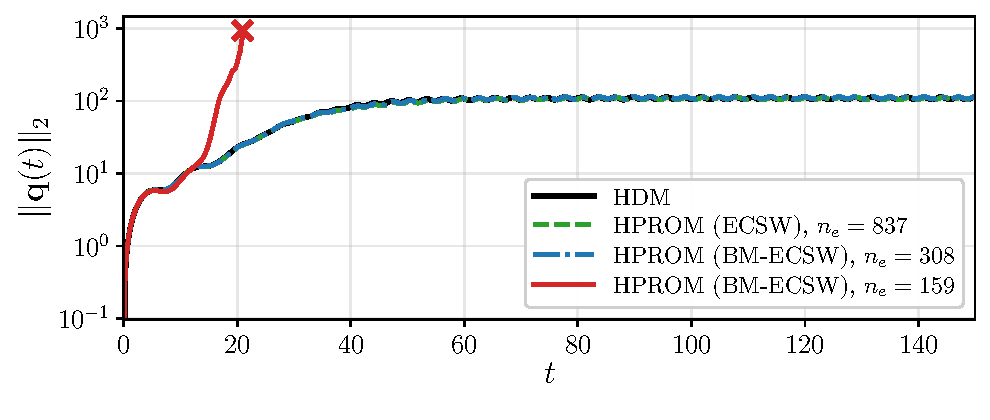
\includegraphics[width=\linewidth]{figures/aerof_bm_coordinate_norm_slides.pdf}
\end{column}
\begin{column}{0.40\textwidth}
\textbf{HPROM (BM-ECSW)}\par
\vspace{4pt}
\begingroup
\centering\rmfamily
\fontsize{8}{9.5}\selectfont
\setlength{\tabcolsep}{2pt}
\renewcommand{\arraystretch}{1.15}
\begin{tabular}{@{}lcc@{}}
\toprule
 & 159 nodes & 308 nodes\\
\midrule
Training tolerance $\tau$ & $10^{-2}$ & $10^{-3}$\\
$\lambda_{\min}/\lambda_{\max}$ & \textcolor{stanfordred}{$-0.019$} & $+0.160$\\
Online result & \shortstack{\textcolor{stanfordred}{Diverges}\\at $t=21$} & \shortstack{Accurate\\to $t=150$}\\
\bottomrule
\end{tabular}\par
\endgroup
\end{column}
\end{columns}
\vspace{3pt}
{\fontsize{7.5}{8.5}\selectfont Ratio: median $\lambda_{\min}/\lambda_{\max}$ of $\operatorname{sym}(\widehat{\matr{J}}_n)$ over assembled correction matrices (Slide~16).}\par
\vspace{6pt}
\textbf{With the same training data, the tighter fit produces an accurate trajectory.}\par
\vspace{3pt}
{\fontsize{8}{9.5}\selectfont The sampled mesh and weights also change; the comparison does not identify the cause of failure.}\par
\vspace{4pt}
\hfill\hyperlink{bmecsw-cylinder-diagnostics}{\beamerbutton{Full trajectories and qualifications}}
\end{frame}


\begin{frame}[t]{Conclusions}
\hypertarget{bmecsw-conclusions}{}
\setlength{\parskip}{0pt}
\begin{itemize}
\fontsize{9.5}{11}\selectfont
\setlength{\itemsep}{4pt}
\setlength{\parsep}{0pt}
\setlength{\topsep}{0pt}
\item \textbf{Substantial savings with comparable accuracy.}
Successful Burgers case: \textbf{$2\,492\rightarrow300$ cells}, approximately
\textbf{$27.5\times$ faster training} and \textbf{$15.4\times$ faster online computation}.
\item \textbf{Additional flexibility changes the inherited guarantees.}
Modal weighting does not automatically preserve one common LSPG objective, a symmetric positive semidefinite
correction matrix, or the mechanical Lagrangian and energy conservation with the same reduced kinetic energy.
\item \textbf{Training and online accuracy are separate checks.}
The Burgers rule with $N_c=90$ fits to $1.28\times10^{-15}$ yet is inaccurate online;
the $N_c=225$ rule achieves comparable trajectory accuracy to classical ECSW.
\item \textbf{Accurate online solutions remain possible.}
The successful BM rule also lacks a common objective. The computations do not isolate which loss causes each failure.
\end{itemize}
\vspace{4pt}
\fontsize{9.5}{11}\selectfont
\textbf{BM offers substantial efficiency gains. Online validation and the structural requirements of the application
remain essential when choosing a hyperreduction rule.}\par
\vspace{5pt}
\hfill\hyperlink{bmecsw-competing-proposals}{\beamerbutton{Competing proposals: $\matr{A}_e$ and grouped weights}}
\end{frame}

% Future main slides belong above this appendix.
\appendix
\bmecswappendixtrue

\begin{frame}[t]{Appendix: individual residual matrices}
\hypertarget{bmecsw-competing-proposals}{}
\fontsize{9}{10.5}\selectfont
\setlength{\parskip}{0pt}
\setlength{\abovedisplayskip}{1pt}
\setlength{\belowdisplayskip}{1pt}
\setlength{\abovedisplayshortskip}{1pt}
\setlength{\belowdisplayshortskip}{1pt}
\textbf{New freedom: one matrix per cell, acting on its HDM residual components.}
\[
  \vect{F}_A(\vect{q})=\widetilde{\vect{r}}_n^A
  =\sum\nolimits_{e\in\widetilde{\mathcal E}}\matr{W}_e^T\matr{A}_e\vect{r}_e.
\]
BM weights reduced equations after projection. Here, $\matr{A}_e$ weights the HDM residual before projection.\par
$\matr{W}_e=\partial\vect{r}_e/\partial\vect{q}$; $\matr{A}_e=\matr{A}_e^T\succeq0$ is trained offline and fixed online.\par
\vspace{2pt}
\textbf{Burgers: two residual components per cell, with separate weights and one cross-weight.}
\[
  \matr{A}_e\vect{r}_e
  =\begin{bmatrix}a_e&b_e\\b_e&c_e\end{bmatrix}
   \begin{bmatrix}r_{u,e}\\r_{v,e}\end{bmatrix}
  =\begin{bmatrix}
    a_e r_{u,e}+b_e r_{v,e}\\
    b_e r_{u,e}+c_e r_{v,e}
   \end{bmatrix}.
\]
\begin{itemize}
\setlength{\itemsep}{0pt}
\setlength{\topsep}{0pt}
\item $a_e,c_e$: weights for the two HDM residual components.
\item $b_e$: couples the $u$ and $v$ residuals \textbf{within the same cell}.
\end{itemize}
{\fontsize{8}{9.5}\selectfont Three independent entries per cell, constrained by $a_e,c_e\geq0$ and $b_e^2\leq a_ec_e$.}\par
\vspace{2pt}
\textbf{The complete vector comes from one common objective:}
\[
  \Phi_A(\vect{q})=\tfrac12\sum\nolimits_{e\in\widetilde{\mathcal E}}
    \vect{r}_e^T\matr{A}_e\vect{r}_e,
  \qquad \nabla_{\vect{q}}\Phi_A=\vect{F}_A.
\]
Its Gauss--Newton correction matrix is symmetric positive semidefinite:
\[
  \widehat{\matr{J}}_n^A
  =\sum\nolimits_{e\in\widetilde{\mathcal E}}\matr{W}_e^T\matr{A}_e\matr{W}_e\succeq0.
\]
$\matr{A}_e=\xi_e\matr{I}$ recovers classical ECSW.\par
\vfill\hfill
\hyperlink{bmecsw-grouped-proposal}{\beamerbutton{Grouped matrices}}
\quad\hyperlink{bmecsw-conclusions}{\beamerreturnbutton{Back to conclusions}}
\end{frame}

\begin{frame}[t]{Appendix: grouped residual matrices}
\hypertarget{bmecsw-grouped-proposal}{}
\fontsize{9}{10.5}\selectfont
\setlength{\parskip}{0pt}
\setlength{\abovedisplayskip}{1pt}
\setlength{\belowdisplayskip}{1pt}
\setlength{\abovedisplayshortskip}{1pt}
\setlength{\belowdisplayshortskip}{1pt}
\textbf{New freedom: cross-weights between residual components of different cells.}
\[
  \vect{F}_{\mathcal P}(\vect{q})=\widetilde{\vect{r}}_n^{\mathcal P}
  =\sum\nolimits_{P\in\mathcal P}\matr{W}_P^T\matr{A}_P\vect{R}_P.
\]
$\vect{R}_P$ stacks the residuals in group $P$; $\matr{W}_P=\partial\vect{R}_P/\partial\vect{q}$.\par
Sampled groups are selected and matrices $\matr{A}_P=\matr{A}_P^T\succeq0$ fitted offline; both are fixed online.\par
\vspace{2pt}
\textbf{For a group of two cells, the matrix has the following blocks:}
\[
  \vect{R}_P=\begin{bmatrix}\vect{r}_{e_1}\\\vect{r}_{e_2}\end{bmatrix},
  \qquad
  \matr{A}_P=\begin{bmatrix}
    \matr{A}_{P,11}&\textcolor{stanfordred}{\matr{A}_{P,12}}\\
    \textcolor{stanfordred}{\matr{A}_{P,12}^T}&\matr{A}_{P,22}
  \end{bmatrix}.
\]
\begin{itemize}
\setlength{\itemsep}{0pt}
\setlength{\topsep}{0pt}
\item Diagonal blocks: weight and couple residual components \textbf{within each cell}.
\item Off-diagonal blocks: couple residual components \textbf{between different cells}.
\end{itemize}
Setting $\matr{A}_{P,12}=\matr{0}$ recovers separate cell matrices.\par
\vspace{2pt}
\textbf{These cross-weights also preserve one common objective:}
\[
  \Phi_{\mathcal P}(\vect{q})=\tfrac12\sum\nolimits_{P\in\mathcal P}
    \vect{R}_P^T\matr{A}_P\vect{R}_P,
  \qquad \nabla_{\vect{q}}\Phi_{\mathcal P}=\vect{F}_{\mathcal P}.
\]
\[
  \widehat{\matr{J}}_n^{\mathcal P}
  =\sum\nolimits_{P\in\mathcal P}\matr{W}_P^T\matr{A}_P\matr{W}_P\succeq0
  \quad\text{(symmetric positive semidefinite).}
\]
{\fontsize{8}{9.5}\selectfont\textbf{Compare against ECSW and BM:} sampled cells, training cost, online time and trajectory accuracy.\par
Experimental competitors: cost and mesh gains remain open. Physical energy conservation is not established.}\par
\vfill\hfill
\hyperlink{bmecsw-competing-proposals}{\beamerreturnbutton{Individual matrices}}
\quad\hyperlink{bmecsw-conclusions}{\beamerreturnbutton{Back to conclusions}}
\end{frame}

\begin{frame}{Appendix: affine approximation and LSPG}
\small
\setlength{\abovedisplayskip}{6pt}
\setlength{\belowdisplayskip}{6pt}
\setlength{\abovedisplayshortskip}{6pt}
\setlength{\belowdisplayshortskip}{6pt}
\textbf{Affine trial space:} fixed $\vect{u}_{\mathrm{ref}}$ and $\matr{V}$; unknown coordinates $\vect{q}$.
\[
  \widetilde{\vect{u}}(\vect{q})
  =\vect{u}_{\mathrm{ref}}+\matr{V}\vect{q},
  \qquad
  \matr{V}\in\mathbb R^{N\times n},
  \qquad n\ll N.
\]

With $\vect{r}(\vect{q}):=\vect{r}^{m+1}(\widetilde{\vect{u}}(\vect{q}))$,
LSPG solves at each time step:
\[
  \vect{q}^{\star}\in
  \underset{\vect{q}\in\mathbb R^n}{\arg\min}\;\Phi(\vect{q}),
  \qquad
  \Phi(\vect{q})=\frac12\left\|\vect{r}(\vect{q})\right\|_2^2.
\]

\textbf{Common scalar objective:} one residual-error measure for all coordinates.

\textbf{To impose stationarity:} differentiate the \textbf{same scalar objective} $\Phi$
with respect to every coordinate, and set all derivatives to zero.
\[
  \vect{r}_n(\vect{q})
  =\nabla_{\vect{q}}\Phi(\vect{q})
  =\matr{W}(\vect{q})^T\vect{r}(\vect{q}),
  \qquad
  \vect{r}_n(\vect{q}^{\star})=\vect{0},
\]
\[
  \matr{W}(\vect{q})
  =\frac{\partial\vect{r}(\vect{q})}{\partial\vect{q}}
  =\matr{J}(\widetilde{\vect{u}}(\vect{q}))\matr{V},
  \qquad
  \matr{J}=\frac{\partial\vect{r}^{m+1}}{\partial\vect{u}}.
\]
{\footnotesize Parameters and known history states are fixed during the solve.}
\end{frame}

\begin{frame}{Appendix: LSPG solution by Gauss--Newton}
\small
\setlength{\abovedisplayskip}{6pt}
\setlength{\belowdisplayskip}{6pt}
\setlength{\abovedisplayshortskip}{6pt}
\setlength{\belowdisplayshortskip}{6pt}
\textbf{From stationarity:} seek
$\nabla_{\vect{q}}\Phi(\vect{q})=\vect{r}_n(\vect{q})=\vect{0}$.

At iteration $k$, let $\vect{r}^{k}=\vect{r}(\vect{q}^{k})$
and $\matr{W}^{k}=\matr{W}(\vect{q}^{k})$.

\textbf{Gauss--Newton:} linearize the HDM residual around $\vect{q}^{k}$:
\[
  \vect{r}(\vect{q}^{k}+\Delta\vect{q})
  \approx\vect{r}^{k}+\matr{W}^{k}\Delta\vect{q}.
\]

\textbf{Local quadratic model:} minimize
$\widehat\Phi_k(\Delta\vect{q})=\tfrac12\|\vect{r}^{k}+\matr{W}^{k}\Delta\vect{q}\|_2^2$
over $\Delta\vect{q}$.

\textbf{Model stationarity:} set
$\nabla_{\Delta\vect{q}}\widehat\Phi_k=\vect{0}$ to obtain the coupled correction:
\[
  \underbrace{[\matr{W}^{k}]^T\matr{W}^{k}}
             _{\displaystyle\widehat{\matr{J}}_n^{k}}
  \Delta\vect{q}^{k}
  =-\underbrace{[\matr{W}^{k}]^T\vect{r}^{k}}
              _{\displaystyle\vect{r}_n(\vect{q}^{k})},
\]
\textbf{Corrected coordinates:}
$\vect{q}^{k+1}=\vect{q}^{k}+\Delta\vect{q}^{k}$.

\vspace{0.4em}
{\footnotesize
  \textbf{Note 1 --- Correction matrix:} symmetric positive semidefinite.\par
  \smallskip
  \textbf{Note 2 --- Gauss--Newton approximation:}
  residual-weighted second derivatives are omitted.
}
\end{frame}

\begin{frame}{Appendix: componentwise ECSW and BM-ECSW}
\small
\setlength{\abovedisplayskip}{6pt}
\setlength{\belowdisplayskip}{6pt}
\setlength{\abovedisplayshortskip}{6pt}
\setlength{\belowdisplayshortskip}{6pt}
\textbf{Vector form:} BM-ECSW weights each component of the projected contributions:
\[
  \widetilde{\vect{r}}_n^{\mathrm{BM}}(\vect{q})
  =\sum_{e\in\widetilde{\mathcal E}}{\color{stanfordred}\matr{D}_e}\vect{g}_e(\vect{q}),
  \qquad
  \matr{D}_e=\operatorname{diag}(\xi_{e,1},\ldots,\xi_{e,n}).
\]

\textbf{Componentwise form} $(i=1,\ldots,n)$:
the scalar weight $\xi_e$ becomes a separate weight $\xi_{e,i}$ for each mode.

\begin{columns}[T,onlytextwidth]
  \begin{column}{0.47\textwidth}
    \textbf{Classical ECSW}

    One weight per entity ($\xi_e\geq0$):
    \[
      \widetilde r_{n,i}^{\mathrm{ECSW}}(\vect{q})
      =\sum_{e\in\widetilde{\mathcal E}}
        {\color{stanfordred}\xi_e}\,g_{e,i}(\vect{q}),
    \]
  \end{column}
  \begin{column}{0.47\textwidth}
    \textbf{BM-ECSW}

    One weight per entity and mode ($\xi_{e,i}\geq0$):
    \[
      \widetilde r_{n,i}^{\mathrm{BM}}(\vect{q})
      =\sum_{e\in\widetilde{\mathcal E}}
        {\color{stanfordred}\xi_{e,i}}\,g_{e,i}(\vect{q}),
    \]
  \end{column}
\end{columns}

\textbf{One shared mesh for all BM modes:} keep an entity if at least one modal weight is positive.

\textbf{Aim:} fit the training contributions with fewer sampled entities.

{\footnotesize Weights are fixed online. Setting $\xi_{e,i}=\xi_e$ for every mode recovers classical ECSW.}
\end{frame}


\begin{frame}{Appendix: crossed derivatives with fixed weights}
\hypertarget{bmecsw-gradient-proof}{}
\footnotesize
\setlength{\parskip}{0pt}
\setlength{\abovedisplayskip}{3pt}
\setlength{\belowdisplayskip}{3pt}
The local functions have continuous second derivatives. The sampled set and weights are fixed.
\begin{columns}[T,onlytextwidth]
\begin{column}{0.49\textwidth}
\textbf{Classical ECSW}
\[
  F_{\mathrm{ECSW},i}
  =\sum\nolimits_{e\in\widetilde{\mathcal E}}\xi_e\frac{\partial\phi_e}{\partial q_i}.
\]
Differentiating the two components gives
\[
\begin{aligned}
  \frac{\partial F_{\mathrm{ECSW},i}}{\partial q_j}
  &=\sum\nolimits_{e\in\widetilde{\mathcal E}}\xi_e
       \frac{\partial^2\phi_e}{\partial q_j\partial q_i},\\[4pt]
  \frac{\partial F_{\mathrm{ECSW},j}}{\partial q_i}
  &=\sum\nolimits_{e\in\widetilde{\mathcal E}}\xi_e
       \frac{\partial^2\phi_e}{\partial q_i\partial q_j}.
\end{aligned}
\]
Subtracting gives
\[
\begin{aligned}
  &\frac{\partial F_{\mathrm{ECSW},i}}{\partial q_j}
   -\frac{\partial F_{\mathrm{ECSW},j}}{\partial q_i}\\[3pt]
  &=\sum\nolimits_{e\in\widetilde{\mathcal E}}\xi_e
    \underbrace{\left[
    \frac{\partial^2\phi_e}{\partial q_j\partial q_i}
    -\frac{\partial^2\phi_e}{\partial q_i\partial q_j}
    \right]}_{=\,0}
    =0.
\end{aligned}
\]
\end{column}
\begin{column}{0.49\textwidth}
\textbf{BM-ECSW}
\[
  F_{\mathrm{BM},i}
  =\sum\nolimits_{e\in\widetilde{\mathcal E}}\xi_{e,i}\frac{\partial\phi_e}{\partial q_i}.
\]
Differentiating the two components gives
\[
\begin{aligned}
  \frac{\partial F_{\mathrm{BM},i}}{\partial q_j}
  &=\sum\nolimits_{e\in\widetilde{\mathcal E}}\xi_{e,i}
       \frac{\partial^2\phi_e}{\partial q_j\partial q_i},\\[4pt]
  \frac{\partial F_{\mathrm{BM},j}}{\partial q_i}
  &=\sum\nolimits_{e\in\widetilde{\mathcal E}}\xi_{e,j}
       \frac{\partial^2\phi_e}{\partial q_i\partial q_j}.
\end{aligned}
\]
The local derivatives agree; subtracting gives
\[
\begin{aligned}
  &\frac{\partial F_{\mathrm{BM},i}}{\partial q_j}
   -\frac{\partial F_{\mathrm{BM},j}}{\partial q_i}\\[3pt]
  &=\underbrace{\sum\nolimits_{e\in\widetilde{\mathcal E}}[\xi_{e,i}-\xi_{e,j}]
    \frac{\partial^2\phi_e}{\partial q_i\partial q_j}}_{\text{not necessarily zero}}.
\end{aligned}
\]
\end{column}
\end{columns}
\vfill\hfill\hyperlink{bmecsw-weighting-comparison}{\beamerreturnbutton{Back to weighting comparison}}
\quad\hyperlink{bmecsw-mechanical-structure}{\beamerreturnbutton{Back to BM mechanics}}
\end{frame}

\begin{frame}{Appendix: deriving the mechanical Lagrangian and conserved energy}
\hypertarget{bmecsw-mechanical-derivation}{}
\fontsize{9}{10.5}\selectfont
\setlength{\parskip}{0pt}
\setlength{\abovedisplayskip}{1pt}
\setlength{\belowdisplayskip}{1pt}
\setlength{\abovedisplayshortskip}{1pt}
\setlength{\belowdisplayshortskip}{1pt}
With $\Phi_{\mathrm{ECSW}}=\sum_{e\in\widetilde{\mathcal E}}\xi_e\phi_e$ and constant symmetric positive definite $\matr{M}_r$,
\[
  \mathcal T_r=\tfrac12\dot{\vect{q}}^T\matr{M}_r\dot{\vect{q}},
  \qquad \widetilde{\mathcal L}_r^{\mathrm{ECSW}}=\mathcal T_r-\Phi_{\mathrm{ECSW}}.
\]
\vspace{3pt}
\begin{columns}[T,onlytextwidth]
\begin{column}{0.48\textwidth}
\textbf{Euler--Lagrange steps}\par
{\fontsize{8}{9}\selectfont\textbf{1. Differentiate in velocity:}}
\[
  \frac{\partial\widetilde{\mathcal L}_r^{\mathrm{ECSW}}}{\partial\dot{\vect{q}}}
  =\matr{M}_r\dot{\vect{q}},
\]
{\fontsize{8}{9}\selectfont\textbf{2. Differentiate in position:}}
\[
  \frac{\partial\widetilde{\mathcal L}_r^{\mathrm{ECSW}}}{\partial\vect{q}}
  =-\nabla_{\vect{q}}\Phi_{\mathrm{ECSW}}=-\vect{F}_{\mathrm{ECSW}}.
\]
{\fontsize{8}{9}\selectfont\textbf{3. Take the time derivative and substitute:}}
\[
  \frac{d}{dt}\left[\frac{\partial\widetilde{\mathcal L}_r^{\mathrm{ECSW}}}{\partial\dot{\vect{q}}}\right]
  -\frac{\partial\widetilde{\mathcal L}_r^{\mathrm{ECSW}}}{\partial\vect{q}}=\vect{0}.
\]
With constant mass, this becomes
\[
  \matr{M}_r\ddot{\vect{q}}+\vect{F}_{\mathrm{ECSW}}=\vect{0}.
\]
\end{column}
\begin{column}{0.48\textwidth}
\textbf{Compute total energy from that same Lagrangian.}
\[
\begin{aligned}
  \widetilde{\mathcal H}_r
  &=\dot{\vect{q}}^T\frac{\partial\widetilde{\mathcal L}_r^{\mathrm{ECSW}}}{\partial\dot{\vect{q}}}
    -\widetilde{\mathcal L}_r^{\mathrm{ECSW}}\\
  &=\dot{\vect{q}}^T\matr{M}_r\dot{\vect{q}}
    -[\tfrac12\dot{\vect{q}}^T\matr{M}_r\dot{\vect{q}}-\Phi_{\mathrm{ECSW}}]\\
  &=\mathcal T_r+\Phi_{\mathrm{ECSW}}.
\end{aligned}
\]
Differentiating along the motion gives
\[
\begin{aligned}
  \frac{d\widetilde{\mathcal H}_r}{dt}
  &=\dot{\vect{q}}^T[\matr{M}_r\ddot{\vect{q}}+\nabla_{\vect{q}}\Phi_{\mathrm{ECSW}}]\\
  &=\dot{\vect{q}}^T[-\vect{F}_{\mathrm{ECSW}}+\vect{F}_{\mathrm{ECSW}}]=0.
\end{aligned}
\]
\end{column}
\end{columns}
\medskip
\textbf{The potential generates the internal vector and makes the energy derivative zero.}\par
\smallskip
{\fontsize{8}{9}\selectfont No external loading; conservation in continuous time. Discrete conservation depends on the time integrator.}
\vfill
\hfill\hyperlink{bmecsw-euler-lagrange-main}{\beamerreturnbutton{Back to Lagrangian structure}}
\quad\hyperlink{bmecsw-mechanical-structure}{\beamerreturnbutton{Back to BM mechanics}}
\end{frame}

\begin{frame}{Appendix: two elements, positive weights, incompatible potential}
\hypertarget{bmecsw-structural-example}{}
\fontsize{9}{10.5}\selectfont
\setlength{\parskip}{0pt}
\setlength{\abovedisplayskip}{1.5pt}
\setlength{\belowdisplayskip}{1.5pt}
\textbf{Keep both elements and their original potential energies:}
\[
  \phi_1=\mathcal V_{1,r}^{\mathrm{int}}=\tfrac12[q_1+q_2]^2,
  \qquad \phi_2=\mathcal V_{2,r}^{\mathrm{int}}=\tfrac12[q_1+2q_2]^2.
\]
Differentiating gives the local internal vectors:
\[
  \nabla_{\vect{q}}\phi_1=\begin{pmatrix}q_1+q_2\\q_1+q_2\end{pmatrix},
  \qquad \nabla_{\vect{q}}\phi_2=\begin{pmatrix}q_1+2q_2\\2[q_1+2q_2]\end{pmatrix}.
\]
\begin{columns}[T,onlytextwidth]
\begin{column}{0.48\textwidth}
\textbf{Classical ECSW:} $\xi_1=\xi_2=1$.
\[
\begin{aligned}
  \vect{F}_{\mathrm{ECSW}}
  &=\nabla_{\vect{q}}\phi_1+\nabla_{\vect{q}}\phi_2\\
  &=\begin{pmatrix}2q_1+3q_2\\3q_1+5q_2\end{pmatrix}.
\end{aligned}
\]
\[
\begin{aligned}
  \frac{\partial F_{\mathrm{ECSW},1}}{\partial q_2}
  &=\frac{\partial[2q_1+3q_2]}{\partial q_2}=3,\\
  \frac{\partial F_{\mathrm{ECSW},2}}{\partial q_1}
  &=\frac{\partial[3q_1+5q_2]}{\partial q_1}=3.
\end{aligned}
\]
The common potential is $\Phi_{\mathrm{ECSW}}=\phi_1+\phi_2$.
\end{column}
\begin{column}{0.48\textwidth}
\textbf{BM-ECSW:} $\matr{D}_1=\operatorname{diag}(1,4)$, $\matr{D}_2=\matr{I}_2$.
\[
\begin{aligned}
  \vect{F}_{\mathrm{BM}}
  &=\begin{pmatrix}q_1+q_2\\4[q_1+q_2]\end{pmatrix}
    +\begin{pmatrix}q_1+2q_2\\2[q_1+2q_2]\end{pmatrix}\\
  &=\begin{pmatrix}2q_1+3q_2\\6q_1+8q_2\end{pmatrix}.
\end{aligned}
\]
\[
\begin{aligned}
  \frac{\partial F_{\mathrm{BM},1}}{\partial q_2}
  &=\frac{\partial[2q_1+3q_2]}{\partial q_2}=3,\\
  \frac{\partial F_{\mathrm{BM},2}}{\partial q_1}
  &=\frac{\partial[6q_1+8q_2]}{\partial q_1}=6.
\end{aligned}
\]
\textbf{No common potential generates this vector.}
\end{column}
\end{columns}
The general difference gives $[1-4]\,1+[1-1]\,2=-3$, agreeing with $3-6$.
\vfill
\hfill\hyperlink{bmecsw-structural-stability}{\beamerbutton{Effect on stability}}
\quad\hyperlink{bmecsw-mechanical-structure}{\beamerreturnbutton{Back to mechanics}}
\end{frame}

\begin{frame}{Appendix: positive modal weights can introduce an unstable mode}
\hypertarget{bmecsw-structural-stability}{}
\fontsize{9}{10.5}\selectfont
\setlength{\parskip}{0pt}
\setlength{\abovedisplayskip}{2pt}
\setlength{\belowdisplayskip}{2pt}
\textbf{The same two-element example has local positive semidefinite stiffness matrices:}
\[
  \matr{K}_{1,r}=\nabla_{\vect{q}}^2\phi_1=\begin{pmatrix}1&1\\1&1\end{pmatrix},
  \qquad \matr{K}_{2,r}=\nabla_{\vect{q}}^2\phi_2=\begin{pmatrix}1&2\\2&4\end{pmatrix}.
\]
\begin{columns}[T,onlytextwidth]
\begin{column}{0.48\textwidth}
\textbf{Classical ECSW: stable oscillatory modes.}
\[
  \matr{K}_r^{\mathrm{ECSW}}=\matr{K}_{1,r}+\matr{K}_{2,r}
  =\begin{pmatrix}2&3\\3&5\end{pmatrix}.
\]
For every nonzero $\vect{z}$,
\[
  \vect{z}^T\matr{K}_r^{\mathrm{ECSW}}\vect{z}
  =[z_1+z_2]^2+[z_1+2z_2]^2>0.
\]
Both squares vanish only for $\vect{z}=\vect{0}$, so the stiffness is positive definite.
\end{column}
\begin{column}{0.48\textwidth}
\textbf{BM-ECSW: a negative stiffness eigenvalue.}
\[
  \matr{K}_r^{\mathrm{BM}}=\matr{D}_1\matr{K}_{1,r}+\matr{K}_{2,r}
  =\begin{pmatrix}2&3\\6&8\end{pmatrix}.
\]
\[
\begin{gathered}
  \det\matr{K}_r^{\mathrm{BM}}=2\cdot8-3\cdot6=-2,\\
  \lambda_-=5-3\sqrt3<0.
\end{gathered}
\]
\end{column}
\end{columns}
\smallskip
For $\matr{M}_r=\matr{I}_2$, the motion $\vect{q}=a(t)\vect{v}_-$ along the negative-eigenvalue mode satisfies
\[
  \ddot a+\lambda_-a=0,
  \qquad a(t)=C_+e^{\sqrt{-\lambda_-}t}+C_-e^{-\sqrt{-\lambda_-}t}.
\]
\smallskip
\textbf{Positive modal weights introduce an exponentially growing mode into a stable classical model.}\par
\smallskip
{\fontsize{8}{9}\selectfont This is a structural counterexample; it does not establish the cause of the flow-computation failures.}
\vfill
\hfill\hyperlink{bmecsw-structural-example}{\beamerreturnbutton{Back to potential test}}
\quad\hyperlink{bmecsw-mechanical-structure}{\beamerreturnbutton{Back to mechanics}}
\end{frame}

\begin{frame}{Appendix: from local residual errors to the sampled LSPG objective}
\hypertarget{bmecsw-lspg-objective-derivation}{}
\fontsize{8.5}{9.5}\selectfont
\setlength{\parskip}{0pt}
\setlength{\abovedisplayskip}{1pt}
\setlength{\belowdisplayskip}{1pt}
\setlength{\abovedisplayshortskip}{1pt}
\setlength{\belowdisplayshortskip}{1pt}
\textbf{Differentiate the local squared residual norm.}
\[
  \phi_e=\tfrac12\vect{r}_e^T\vect{r}_e,
  \qquad \matr{W}_e=\frac{\partial\vect{r}_e}{\partial\vect{q}}.
\]
For each coordinate $q_i$, the product rule gives
\[
\begin{aligned}
  \frac{\partial\phi_e}{\partial q_i}
  &=\tfrac12\left[
    \left[\frac{\partial\vect{r}_e}{\partial q_i}\right]^T\vect{r}_e
    +\vect{r}_e^T\frac{\partial\vect{r}_e}{\partial q_i}\right]
   =\matr{W}_e(:,i)^T\vect{r}_e,\\
  \nabla_{\vect{q}}\phi_e
  &=\tfrac12[\matr{W}_e^T\vect{r}_e+[\vect{r}_e^T\matr{W}_e]^T]
   =\matr{W}_e^T\vect{r}_e.
\end{aligned}
\]
The two scalar terms in the component derivative are equal, canceling the factor $1/2$.\par
\vspace{4pt}
\begin{columns}[T,onlytextwidth]
\begin{column}{0.48\textwidth}
\textbf{Full LSPG}
\[
  \Phi=\sum\nolimits_{e\in\mathcal E}\phi_e
  =\tfrac12\|\vect{r}(\vect{q})\|_2^2.
\]
\[
\begin{aligned}
  \nabla_{\vect{q}}\Phi
  &=\sum\nolimits_{e\in\mathcal E}\nabla_{\vect{q}}\phi_e\\
  &=\sum\nolimits_{e\in\mathcal E}\matr{W}_e^T\vect{r}_e
   =\vect{r}_n=\vect{F}.
\end{aligned}
\]
The residual blocks partition the assembled HDM residual rows.
\end{column}
\begin{column}{0.48\textwidth}
\textbf{Classical ECSW: fixed scalar weights}
\[
  \Phi_{\mathrm{ECSW}}
  =\sum\nolimits_{e\in\widetilde{\mathcal E}}\xi_e\phi_e
  =\tfrac12\sum\nolimits_{e\in\widetilde{\mathcal E}}\xi_e\|\vect{r}_e\|_2^2.
\]
\[
\begin{aligned}
  \nabla_{\vect{q}}\Phi_{\mathrm{ECSW}}
  &=\sum\nolimits_{e\in\widetilde{\mathcal E}}\xi_e\nabla_{\vect{q}}\phi_e\\
  &=\sum\nolimits_{e\in\widetilde{\mathcal E}}\xi_e\matr{W}_e^T\vect{r}_e\\
  &=\widetilde{\vect{r}}_n^{\mathrm{ECSW}}=\vect{F}_{\mathrm{ECSW}}.
\end{aligned}
\]
Its gradient generates every sampled projected equation.
\end{column}
\end{columns}
\vfill
\hfill\hyperlink{bmecsw-lspg-objective}{\beamerreturnbutton{Back to LSPG objective}}
\end{frame}

\begin{frame}{Appendix: LSPG example --- local contributions and objective}
\hypertarget{bmecsw-lspg-example-details}{}
\fontsize{9}{10.5}\selectfont
\setlength{\parskip}{0pt}
\setlength{\abovedisplayskip}{1pt}
\setlength{\belowdisplayskip}{1pt}
\setlength{\abovedisplayshortskip}{1pt}
\setlength{\belowdisplayshortskip}{1pt}
The local functions are $\phi_e=\tfrac12 r_e^2$, with
$r_1=q_1$, $r_2=q_2$, and $r_3=q_1+q_2^2-3$.
Their gradients supply the projected contributions:
\[
  \nabla_{\vect{q}}\phi_e=\matr{W}_e^T r_e,
  \qquad
  \matr{W}_1=(1,0),\quad \matr{W}_2=(0,1),\quad \matr{W}_3=(1,2q_2).
\]
\begin{columns}[T,onlytextwidth]
\begin{column}{0.48\textwidth}
\textbf{Classical ECSW}
\[
\begin{aligned}
 \widetilde{\vect{r}}_n^{\mathrm{ECSW}}
 &=2\begin{pmatrix}r_1\\0\end{pmatrix}
  +3\begin{pmatrix}0\\r_2\end{pmatrix}
  +2\begin{pmatrix}r_3\\2q_2r_3\end{pmatrix}\\[3pt]
 &=\begin{pmatrix}2q_1+2r_3\\3q_2+4q_2r_3\end{pmatrix}.
\end{aligned}
\]
The scalar weights define one common objective:
\[
  \Phi_{\mathrm{ECSW}}
  =\tfrac12\left[2q_1^2+3q_2^2+2r_3^2\right].
\]
Differentiating verifies both components:
\[
\begin{aligned}
  \frac{\partial\Phi_{\mathrm{ECSW}}}{\partial q_1}
  &=2q_1+2r_3,\\
  \frac{\partial\Phi_{\mathrm{ECSW}}}{\partial q_2}
  &=3q_2+4q_2r_3.
\end{aligned}
\]
\end{column}
\begin{column}{0.48\textwidth}
\textbf{BM-ECSW}
\[
\begin{aligned}
 \widetilde{\vect{r}}_n^{\mathrm{BM}}
 &=2\begin{pmatrix}r_1\\0\end{pmatrix}
  +3\begin{pmatrix}0\\r_2\end{pmatrix}
  +\begin{pmatrix}2&0\\0&1\end{pmatrix}
    \begin{pmatrix}r_3\\2q_2r_3\end{pmatrix}\\[3pt]
 &=\begin{pmatrix}2q_1+2r_3\\3q_2+2q_2r_3\end{pmatrix}.
\end{aligned}
\]
The crossed derivatives give
\[
  \frac{\partial\widetilde r_{n,1}^{\mathrm{BM}}}{\partial q_2}
  -\frac{\partial\widetilde r_{n,2}^{\mathrm{BM}}}{\partial q_1}
  =4q_2-2q_2=2q_2.
\]
For $q_2\ne0$, this excludes every common smooth scalar objective locally.\par\vspace{0.5em}
Changing the weight pair of entity 3 from $(2,1)$ to $(2,2)$ recovers the classical vector and objective.
\end{column}
\end{columns}
\vfill\hfill\hyperlink{bmecsw-lspg-example}{\beamerreturnbutton{Back to LSPG example}}
\end{frame}

\begin{frame}{Appendix: the exact BM Jacobian and its approximation}
\hypertarget{bmecsw-bm-jacobian-approximation}{}
\fontsize{9.5}{11}\selectfont
\setlength{\parskip}{0pt}
\setlength{\abovedisplayskip}{2pt}
\setlength{\belowdisplayskip}{2pt}
\setlength{\abovedisplayshortskip}{2pt}
\setlength{\belowdisplayshortskip}{2pt}
\textbf{The online target is the BM projected equation:}
\[
  \widetilde{\vect{r}}_n^{\mathrm{BM}}(\vect{q})
  =\sum\nolimits_{e\in\widetilde{\mathcal E}}\matr{D}_e\matr{W}_e(\vect{q})^T\vect{r}_e(\vect{q})
  =\vect{0}.
\]
With fixed weights, its exact Jacobian differentiates both $\matr{W}_e$ and $\vect{r}_e$:
\[
\begin{aligned}
  \left[\matr{J}_n^{\mathrm{BM}}\right]_{ij}
  &=\frac{\partial\widetilde r_{n,i}^{\mathrm{BM}}}{\partial q_j}\\
  &=\underbrace{\sum\nolimits_{e\in\widetilde{\mathcal E}}\xi_{e,i}
      \matr{W}_e(:,i)^T\matr{W}_e(:,j)}_{
      [\widehat{\matr{J}}_n^{\mathrm{BM}}]_{ij}}
   +\underbrace{\sum\nolimits_{e\in\widetilde{\mathcal E}}\xi_{e,i}
      \vect{r}_e^T\frac{\partial^2\vect{r}_e}{\partial q_j\partial q_i}}_{
      \text{residual-weighted second derivatives}}.
\end{aligned}
\]
\textbf{Retaining only the first term gives the matrix used online:}
\[
  \widehat{\matr{J}}_n^{\mathrm{BM}}
  =\sum\nolimits_{e\in\widetilde{\mathcal E}}\matr{D}_e\matr{W}_e^T\matr{W}_e,
  \qquad
  \widehat{\matr{J}}_n^{\mathrm{BM}}\Delta\vect{q}^{\mathrm{BM}}
  =-\widetilde{\vect{r}}_n^{\mathrm{BM}}.
\]
This is an approximate Newton correction for the BM projected equations. The omission of residual-weighted second derivatives explains the Gauss--Newton-type designation; it does not establish a common least-squares objective.\par
\vspace{0pt}
{\fontsize{8}{9}\selectfont Classical Gauss--Newton minimizes its quadratic model; a full step does not guarantee a decrease in the nonlinear objective. Gradient compatibility is tested with the exact Jacobian, not its first-derivative approximation.}
\vfill\hfill\hyperlink{bmecsw-online-interpretation}{\beamerreturnbutton{Back to online correction}}
\end{frame}

\begin{frame}{Appendix: correction-matrix entries and quadratic forms}
\hypertarget{bmecsw-correction-calculations}{}
\fontsize{9}{10.5}\selectfont
\setlength{\parskip}{0pt}
\setlength{\abovedisplayskip}{2pt}
\setlength{\belowdisplayskip}{2pt}
\setlength{\abovedisplayshortskip}{2pt}
\setlength{\belowdisplayshortskip}{2pt}
\textbf{With fixed diagonal $\matr{D}_e$, the crossed BM entries are}
\[
\begin{aligned}
 \left[\widehat{\matr{J}}_n^{\mathrm{BM}}\right]_{ij}
 &=\sum\nolimits_{e\in\widetilde{\mathcal E}}\xi_{e,i}\matr{W}_e(:,i)^T\matr{W}_e(:,j),\\
 \left[\widehat{\matr{J}}_n^{\mathrm{BM}}\right]_{ji}
 &=\sum\nolimits_{e\in\widetilde{\mathcal E}}\xi_{e,j}\matr{W}_e(:,j)^T\matr{W}_e(:,i).
\end{aligned}
\]
The two local inner products agree, so subtraction gives
\[
 [\widehat{\matr{J}}_n^{\mathrm{BM}}]_{ij}
 -[\widehat{\matr{J}}_n^{\mathrm{BM}}]_{ji}
 =\sum\nolimits_{e\in\widetilde{\mathcal E}}[\xi_{e,i}-\xi_{e,j}]
 \matr{W}_e(:,i)^T\matr{W}_e(:,j).
\]
\textbf{The quadratic forms follow by grouping the products:}
\[
\begin{aligned}
 \vect{z}^T\widehat{\matr{J}}_n^{\mathrm{ECSW}}\vect{z}
 &=\sum\nolimits_{e\in\widetilde{\mathcal E}}\xi_e
 [\matr{W}_e\vect{z}]^T[\matr{W}_e\vect{z}]
 =\sum\nolimits_{e\in\widetilde{\mathcal E}}\xi_e\|\matr{W}_e\vect{z}\|_2^2\geq0,\\
 \vect{z}^T\widehat{\matr{J}}_n^{\mathrm{BM}}\vect{z}
 &=\sum\nolimits_{e\in\widetilde{\mathcal E}}\vect{z}^T\matr{D}_e\matr{W}_e^T\matr{W}_e\vect{z}
 =\sum\nolimits_{e\in\widetilde{\mathcal E}}
 [\matr{W}_e\matr{D}_e\vect{z}]^T[\matr{W}_e\vect{z}].
\end{aligned}
\]
\textbf{A scalar equals its transpose. Averaging both forms gives}
\[
\begin{aligned}
 \vect{z}^T\widehat{\matr{J}}_n\vect{z}
 &=\tfrac12[\vect{z}^T\widehat{\matr{J}}_n\vect{z}
            +\vect{z}^T\widehat{\matr{J}}_n^T\vect{z}]\\
 &=\vect{z}^T\operatorname{sym}(\widehat{\matr{J}}_n)\vect{z},
 \qquad \operatorname{sym}(\widehat{\matr{J}}_n)
 =\tfrac12[\widehat{\matr{J}}_n+\widehat{\matr{J}}_n^T].
\end{aligned}
\]
For $\operatorname{sym}(\widehat{\matr{J}}_n)\vect{v}=\lambda\vect{v}$,
$\vect{v}^T\widehat{\matr{J}}_n\vect{v}=\lambda\|\vect{v}\|_2^2$.
Setting $\matr{D}_e=\xi_e\matr{I}_n$ recovers the classical matrix.\par
\vfill\hfill\hyperlink{bmecsw-correction-properties}{\beamerreturnbutton{Back to correction matrices}}
\end{frame}

\begin{frame}{Appendix: positive eigenvalues and temporary perturbation growth}
\hypertarget{bmecsw-positive-eigenvalue-example}{}
\fontsize{9}{10.5}\selectfont
\setlength{\parskip}{0pt}
\setlength{\abovedisplayskip}{2pt}
\setlength{\belowdisplayskip}{2pt}
\setlength{\abovedisplayshortskip}{2pt}
\setlength{\belowdisplayshortskip}{2pt}
\textbf{Hold the matrix fixed in the auxiliary model $\dot{\vect{z}}=-\widehat{\matr{J}}_n\vect{z}$.}
\[
 \frac{d}{dt}\,\tfrac12\|\vect{z}\|_2^2
 =\vect{z}^T\dot{\vect{z}}
 =-\vect{z}^T\widehat{\matr{J}}_n\vect{z}
 =-\vect{z}^T\operatorname{sym}(\widehat{\matr{J}}_n)\vect{z}.
\]
A positive quadratic form decreases the perturbation norm; a negative one initially increases it.\par
Using $\matr{W}_1=(1,0)$, $\matr{W}_2=(0,1)$, and $\matr{W}_3=(1,1)$ gives:
\begin{columns}[T,onlytextwidth]
\begin{column}{0.48\textwidth}
\textbf{Classical ECSW}
\[
 \vect{\xi}=\begin{pmatrix}1\\1\\4\end{pmatrix},
 \qquad \widehat{\matr{J}}_n^{\mathrm{ECSW}}
 =\begin{pmatrix}5&4\\4&5\end{pmatrix}.
\]
The matrix is symmetric positive definite, with eigenvalues $1$ and $9$.\par
For $\vect{z}=(1,-2)^T$,
\[
 \vect{z}^T\widehat{\matr{J}}_n^{\mathrm{ECSW}}\vect{z}=9,
 \qquad \left.\frac{d}{dt}\,\tfrac12\|\vect{z}\|_2^2\right|_{t=0}=-9.
\]
The perturbation norm decreases from the start.
\end{column}
\begin{column}{0.48\textwidth}
\textbf{BM-ECSW}
\[
 \matr{\Xi}=\begin{pmatrix}1&1\\1&1\\8&0\end{pmatrix},
 \qquad \widehat{\matr{J}}_n^{\mathrm{BM}}
 =\begin{pmatrix}9&8\\0&1\end{pmatrix}.
\]
The eigenvalues are again $1$ and $9$, but
\[
 \operatorname{sym}(\widehat{\matr{J}}_n^{\mathrm{BM}})
 =\begin{pmatrix}9&4\\4&1\end{pmatrix},
 \quad \lambda=5\pm4\sqrt2.
\]
For the same $\vect{z}$, the quadratic form is $-3$, so $\left.\tfrac{d}{dt}\tfrac12\|\vect{z}\|_2^2\right|_{t=0}=+3$.
\end{column}
\end{columns}
\vspace{3pt}
\textbf{Both auxiliary models eventually decay; BM can amplify the perturbation temporarily.}\par
{\fontsize{8}{9}\selectfont The symmetric part has determinant $-7$ and one negative eigenvalue. The weights are nonnegative; entity 3 has zero weight in the second component. This auxiliary equation is not the HPROM physical evolution.}\par
\vfill\hfill\hyperlink{bmecsw-correction-properties}{\beamerreturnbutton{Back to correction matrices}}
\end{frame}


\begin{frame}[t]{Appendix: Burgers gradient test and trajectories}
\hypertarget{bmecsw-burgers-diagnostics}{}
\fontsize{8}{9}\selectfont
\setlength{\parskip}{0pt}
The crossed derivatives are tested at every computed state: three parameters, 500 steps each.\par
\vspace{3pt}
\begingroup
\centering\rmfamily
\setlength{\tabcolsep}{4pt}
\renewcommand{\arraystretch}{1.05}
\begin{tabular}{@{}lrrr@{}}
\toprule
Model & $N_c$ & $\|\matr{J}_n-\matr{J}_n^T\|_F/\|\matr{J}_n\|_F$ & Nonsymmetric\\
\midrule
HPROM (ECSW) & 90 & $8.95\times10^{-17}$ & $0/1\,500$\\
HPROM (ECSW) & 225 & $8.74\times10^{-17}$ & $0/1\,500$\\
HPROM (BM-ECSW) & 90 & 1.099 & $1\,500/1\,500$\\
HPROM (BM-ECSW) & 225 & 0.434 & $1\,500/1\,500$\\
\bottomrule
\end{tabular}
\par
\endgroup
\vspace{3pt}
\centering
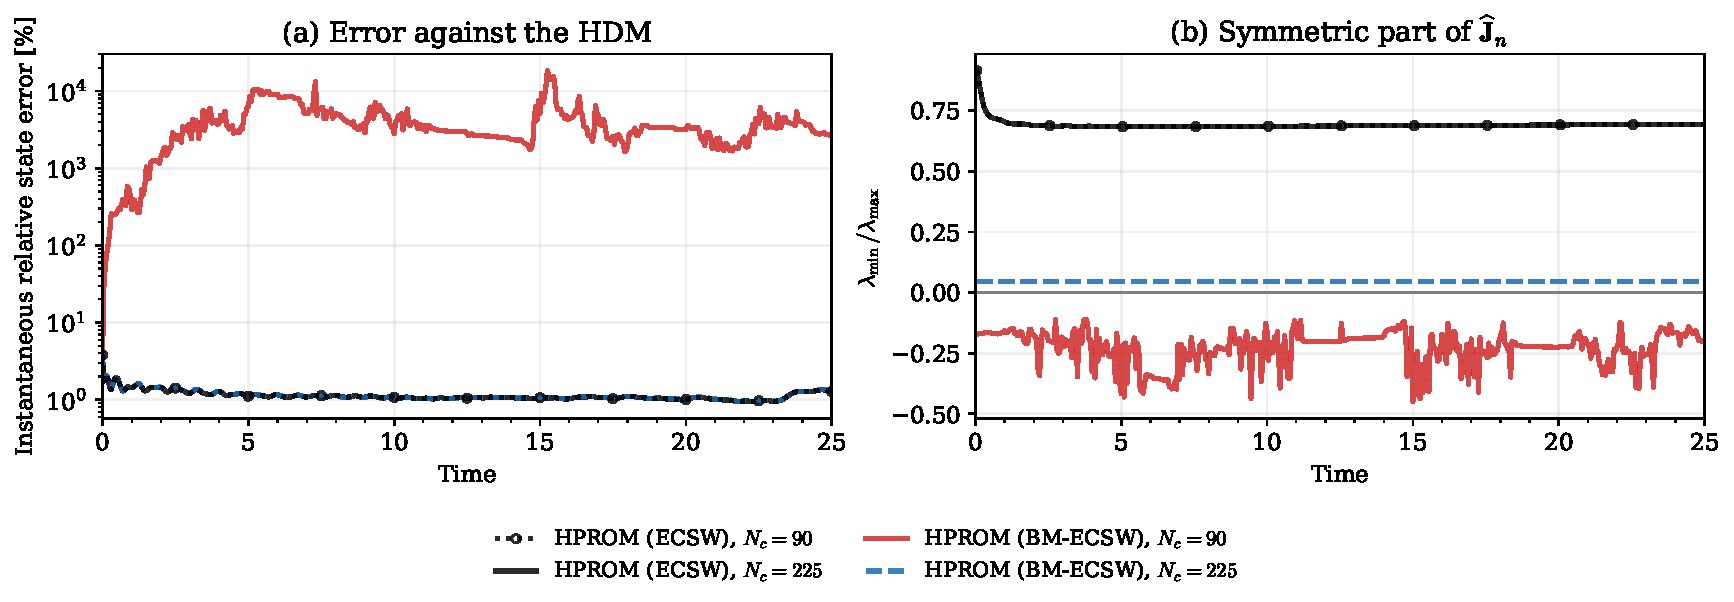
\includegraphics[width=0.79\linewidth]{figures/burgers_bm_stability.pdf}\par
{\fontsize{7.5}{8.5}\selectfont Trajectories at $\vect{\mu}=(4.56,0.019)$; correction matrices at the first iterate of each step.}\par
\hfill\hyperlink{bmecsw-burgers-evidence}{\beamerreturnbutton{Back to Burgers}}
\end{frame}

\begin{frame}{Appendix: accurately solved Burgers steps}
\hypertarget{bmecsw-burgers-step-accuracy}{}
\fontsize{9}{10.5}\selectfont
\setlength{\parskip}{0pt}
\textbf{Test the equations separately from accumulated trajectory error.}\par
\vspace{5pt}
Reference PROM: full-mesh residual, same 96-mode ROB; 20 steps at $\vect{\mu}=(4.56,0.019)$.\par
\vspace{5pt}
At steps 1, 5, and 20, every model receives the same previous PROM state and solves its own projected equations to a relative residual below $10^{-11}$.\par
\vspace{6pt}
\textbf{First-step results}\par
\vspace{4pt}
\begingroup
\centering\rmfamily
\fontsize{8.5}{10}\selectfont
\setlength{\tabcolsep}{5pt}
\renewcommand{\arraystretch}{1.12}
\begin{tabular}{@{}lrrr@{}}
\toprule
Model & $\lambda_{\min}/\lambda_{\max}$ & $\kappa_2(\widehat{\matr{J}}_n)$ & State error [\%]\\
\midrule
PROM & $+0.915$ & 1.09 & 0\\
HPROM (ECSW), $N_c=90$ & $+0.915$ & 1.09 & $4.06\times10^{-4}$\\
HPROM (ECSW), $N_c=225$ & $+0.915$ & 1.09 & $9.17\times10^{-6}$\\
HPROM (BM-ECSW), $N_c=90$ & $-0.172$ & 3\,233.39 & 30.626\\
HPROM (BM-ECSW), $N_c=225$ & $+0.044$ & 13.40 & 0.048\\
\bottomrule
\end{tabular}
\par
\endgroup
\vspace{4pt}
{\fontsize{8}{9}\selectfont State errors are against the PROM; matrix ratios and condition numbers are at the common initial guess.}\par
\vspace{7pt}
\textbf{BM can satisfy its equations accurately and still produce an inaccurate state.}\par
Failure of the nonlinear solver alone cannot explain the unsuccessful trajectory.\par
\vfill\hfill\hyperlink{bmecsw-burgers-evidence}{\beamerreturnbutton{Back to Burgers}}
\end{frame}

\begin{frame}[t]{Appendix: cylinder trajectories and matrix diagnostics}
\hypertarget{bmecsw-cylinder-diagnostics}{}
\fontsize{8}{9}\selectfont
\setlength{\parskip}{0pt}
\begin{columns}[T,onlytextwidth]
\begin{column}{0.46\textwidth}
\centering
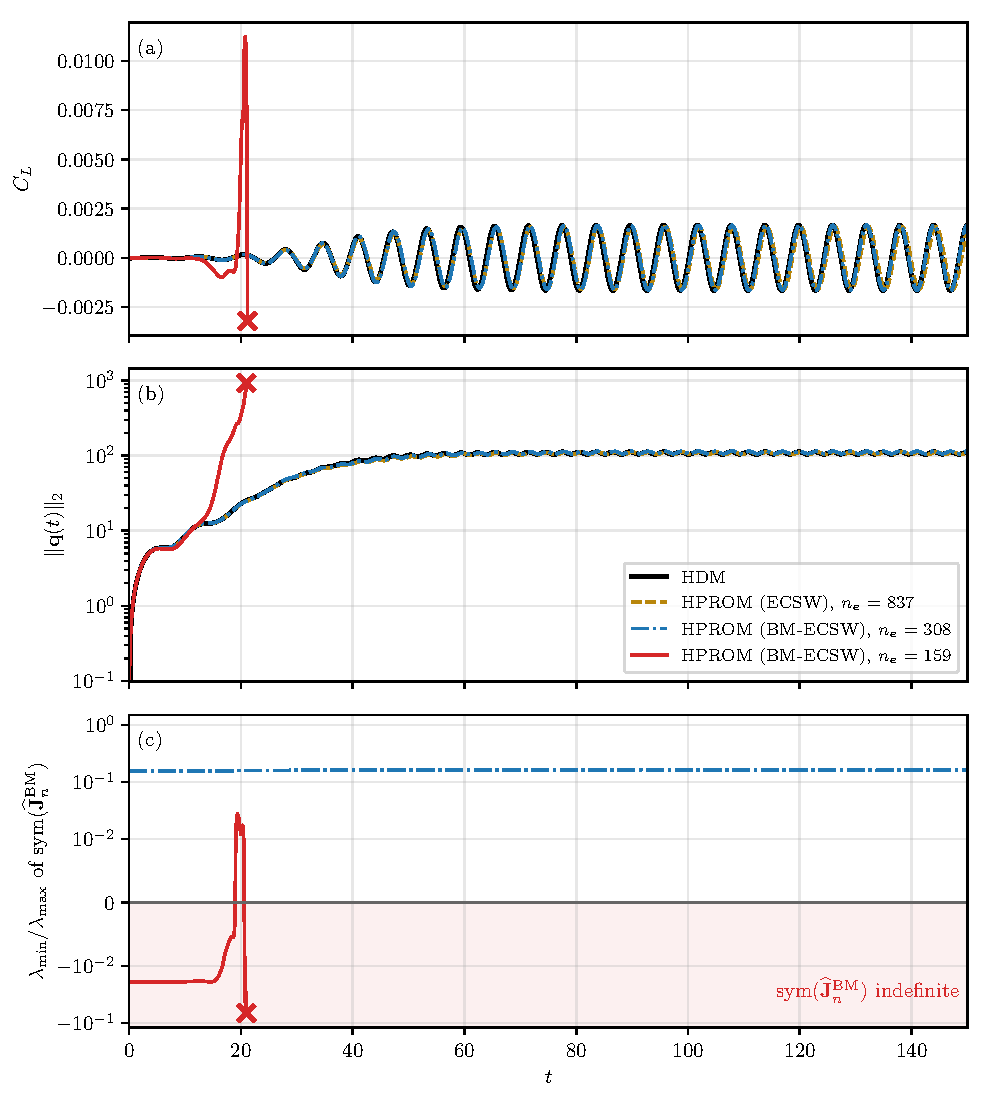
\includegraphics[height=0.72\textheight]{figures/aerof_bm_divergence.pdf}
\end{column}
\begin{column}{0.51\textwidth}
\textbf{Same ROB ($n=96$); test at $\mathrm{Re}=100$.}\par
\vspace{4pt}
\textbf{159 nodes, $\tau=10^{-2}$}\par
Median symmetric-part ratio: $-0.019$; indefinite in 210 of 226 recorded matrices. The run stops at $t=21$ with negative pressures.\par
\vspace{4pt}
\textbf{308 nodes, $\tau=10^{-3}$}\par
Median ratio: $+0.160$; positive definite in all 1\,500 recorded matrices. The trajectory remains close to the HDM and classical ECSW.\par
\vspace{4pt}
\textbf{Additional check: eigenvalues of $\widehat{\matr{J}}_n$.}\par
Both rules have positive eigenvalue real parts at every recorded assembly, despite their different outcomes.\par
\vspace{4pt}
\textbf{The ratio alone does not establish stability.}\par
A 174-node BM rule diverges at $t=41.5$, although this part is positive definite from $t=25$ until failure.\par
\vspace{4pt}
Classical rules restricted to 159 and 174 nodes also diverge, at $t=56$ and $80$. A sufficiently small classical mesh can fail as well.
\end{column}
\end{columns}
\vfill\hfill\hyperlink{bmecsw-cylinder-evidence}{\beamerreturnbutton{Back to cylinder}}
\end{frame}


\begin{frame}[t]{Appendix: initialization and stopping (lines 1--5, 13--14)}
\small
\hypertarget{ecsw-line-1}{}%
\hypertarget{ecsw-line-2}{}%
\hypertarget{ecsw-line-3}{}%
\hypertarget{ecsw-line-4}{}%
\hypertarget{ecsw-line-5}{}%
\hypertarget{ecsw-line-13}{}%
\hypertarget{ecsw-line-14}{}%
\textbf{Start with no sampled contributions:}
\[
  k=0,\qquad \mathcal I^0=\varnothing,\qquad
  \mathcal Z^0=\mathcal E,\qquad \vect{\xi}^{\,0}=\vect{0}.
\]
$\mathcal I^k$ contains the selected entities;
$\mathcal Z^k=\mathcal E\setminus\mathcal I^k$ contains the remaining candidates.

\textbf{Cubature fitting residual:} measure the difference from the full target:
\[
  \vect{h}^{\,k}=\vect{b}-\matr{G}\vect{\xi}^{\,k},
  \qquad \vect{h}^{\,0}=\vect{b}.
\]

\textbf{Training accuracy:} continue selection while
\[
  \eta^k=\frac{\|\vect{h}^{\,k}\|_2}{\|\vect{b}\|_2}>\tau.
\]
After each refit, increase $k$ and check the updated fitting error.
The tolerance controls the accuracy of the cubature fit on the training data.
\BackToClassicalAlgorithm
\end{frame}

\begin{frame}[t]{Appendix: the correlation score (line 6)}
\small
\setlength{\abovedisplayskip}{4pt}
\setlength{\belowdisplayskip}{4pt}
\setlength{\abovedisplayshortskip}{4pt}
\setlength{\belowdisplayshortskip}{4pt}
\hypertarget{ecsw-line-6}{}%
\textbf{Training objective:} $F(\vect{\xi})=\tfrac12\|\matr{G}\vect{\xi}-\vect{b}\|_2^2$.

\textbf{Expand the quadratic:}
\[
  \begin{aligned}
    2F(\vect{\xi})
    &=[\matr{G}\vect{\xi}-\vect{b}]^T[\matr{G}\vect{\xi}-\vect{b}]\\
    &=\vect{\xi}^T\matr{G}^T\matr{G}\vect{\xi}
      -2\vect{\xi}^T\matr{G}^T\vect{b}+\vect{b}^T\vect{b}.
  \end{aligned}
\]

\textbf{Differentiate with respect to the weights:}
\[
  \nabla_{\vect{\xi}}F(\vect{\xi}^{\,k})
  =\matr{G}^T\matr{G}\vect{\xi}^{\,k}-\matr{G}^T\vect{b}
  =-\matr{G}^T\vect{h}^{\,k}.
\]

\textbf{Hence the score is the negative fitting gradient:}
\[
  \vect{\mu}^{\,k}=\matr{G}^T\vect{h}^{\,k}
  =-\nabla_{\vect{\xi}}F(\vect{\xi}^{\,k}),
  \qquad \vect{h}^{\,k}=\vect{b}-\matr{G}\vect{\xi}^{\,k}.
\]
{\footnotesize For column $\vect{g}_e=\matr{G}(:,e)$, $\mu_e^k=\vect{g}_e^T\vect{h}^{\,k}$.
For an unselected entity, a positive score means that increasing its zero weight initially decreases $F$.}
\BackToClassicalAlgorithm
\end{frame}

\begin{frame}[t]{Appendix: selecting the largest score (line 7)}
\small
\hypertarget{ecsw-line-7}{}%
\textbf{Feasible candidate:} for $e\in\mathcal Z^k$, the current weight is zero.
Increase it by $t\geq0$, keeping the other weights fixed:
\[
  \vect{\xi}(t)=\vect{\xi}^{\,k}+t\vect{e}_e,
  \qquad \matr{G}\vect{e}_e=\vect{g}_e,
\]
Here $\vect{e}_e$ is the unit vector for weight $e$,
$\vect{h}^{\,k}=\vect{b}-\matr{G}\vect{\xi}^{\,k}$,
and $\mu_e^k=\vect{g}_e^T\vect{h}^{\,k}$.

\textbf{Effect on the fitting objective}
$F(\vect{\xi})=\tfrac12\|\matr{G}\vect{\xi}-\vect{b}\|_2^2$:
\[
  F(\vect{\xi}^{\,k}+t\vect{e}_e)
  =F(\vect{\xi}^{\,k})-t\mu_e^k
   +\frac{t^2}{2}\|\vect{g}_e\|_2^2.
\]

\textbf{Compare initial slopes for the same weight increment:}
\[
  \left.\frac{d}{dt}F(\vect{\xi}^{\,k}+t\vect{e}_e)\right|_{t=0}
  =-\mu_e^k,
  \qquad e^k\in\arg\max_{e\in\mathcal Z^k}\mu_e^k.
\]
The largest positive score gives the greatest initial decrease.
{\footnotesize This initial-slope criterion does not guarantee the largest improvement after the NNLS refit.}
\BackToClassicalAlgorithm
\end{frame}

\begin{frame}[t]{Appendix: selected sets and NNLS refitting (lines 8--12)}
\small
\hypertarget{ecsw-line-8}{}%
\hypertarget{ecsw-line-9}{}%
\hypertarget{ecsw-line-10}{}%
\hypertarget{ecsw-line-11}{}%
\hypertarget{ecsw-line-12}{}%
\textbf{Enlarge the working set and update the remaining candidates:}
\[
  \mathcal I^{k+1}=\mathcal I^k\cup\{e^k\},
  \qquad \mathcal Z^{k+1}=\mathcal E\setminus\mathcal I^{k+1}.
\]

\textbf{Refit all selected weights against the original target $\vect{b}$:}
\[
  \vect{\xi}^{\,k+1}_{\mathcal I^{k+1}}\in
  \underset{\vect{z}\geq\vect{0}}{\arg\min}
  \frac12\|\matr{G}_{\mathcal I^{k+1}}\vect{z}-\vect{b}\|_2^2,
  \qquad \vect{\xi}^{\,k+1}_{\mathcal Z^{k+1}}=\vect{0}.
\]
Existing weights may increase, decrease, or become zero.
Every unselected entity retains zero weight.

\textbf{Then measure the error of the new complete rule:}
\[
  \vect{h}^{\,k+1}=\vect{b}-\matr{G}\vect{\xi}^{\,k+1}.
\]
This updated fitting residual determines the next scores and the stopping test.
\BackToClassicalAlgorithm
\end{frame}

\begin{frame}[t]{Appendix: the positive support defines the mesh (lines 15--16)}
\small
\hypertarget{ecsw-line-15}{}%
\hypertarget{ecsw-line-16}{}%
\textbf{An NNLS refit can assign zero weight to a selected entity.}
The final sampled mesh therefore contains the positive-weight entities:
\[
  \widetilde{\mathcal E}
  =\{e\in\mathcal E:\xi_e^{\,k}>0\}
  \subseteq\mathcal I^k.
\]

\textbf{Only these entities contribute to the sampled projected residual:}
\[
  \widetilde{\vect{r}}_n^{\mathrm{ECSW}}(\vect{q})
  =\sum_{e\in\widetilde{\mathcal E}}\xi_e^{\,k}\vect{g}_e(\vect{q}).
\]

\textbf{Return both parts of the cubature rule:}
the full weight vector $\vect{\xi}^{\,k}$ and its positive support $\widetilde{\mathcal E}$.
The weights are fixed during the online simulation.

\textbf{Mesh size is an output:} $|\widetilde{\mathcal E}|$ follows from the trained rule.
\BackToClassicalAlgorithm
\end{frame}

\begin{frame}[t]{Appendix: BM initialization and stopping (lines 1--3, 13--14)}
\small
\setlength{\abovedisplayskip}{6pt}
\setlength{\belowdisplayskip}{6pt}
\hypertarget{bm-ecsw-line-1}{}%
\hypertarget{bm-ecsw-line-2}{}%
\hypertarget{bm-ecsw-line-3}{}%
\hypertarget{bm-ecsw-line-13}{}%
\hypertarget{bm-ecsw-line-14}{}%
\textbf{One shared working set, initially empty:}
\[
  k=0,\qquad \mathcal I^0=\varnothing,\qquad
  \mathcal Z^0=\mathcal E.
\]
\textbf{Initialize every mode with zero weights:}
\[
  \vect{\xi}^{[i],0}=\vect{0},\qquad
  \vect{h}^{[i],0}=\vect{b}^{[i]},\qquad i=1,\ldots,n.
\]
At later iterations, $\vect{h}^{[i],k}=\vect{b}^{[i]}-\matr{G}^{[i]}\vect{\xi}^{[i],k}$.

\textbf{Check one aggregate training error:} continue selection while
\[
  [\eta^k]^2=
  \frac{\sum_i\|\vect{h}^{[i],k}\|_2^2}
       {\sum_i\|\vect{b}^{[i]}\|_2^2}>\tau^2.
\]
The denominator is positive by assumption. Individual modal targets may be zero;
no separate relative tolerance is imposed on each mode.
\BackToBMAlgorithm
\end{frame}

\begin{frame}[t]{Appendix: BM correlation score (line 4)}
\small
\setlength{\abovedisplayskip}{3pt}
\setlength{\belowdisplayskip}{3pt}
\setlength{\abovedisplayshortskip}{3pt}
\setlength{\belowdisplayshortskip}{3pt}
\hypertarget{bm-ecsw-line-4}{}%
\textbf{Expand the offline fitting objective:}
$\matr{\Xi}=[\vect{\xi}^{[1]}\ \cdots\ \vect{\xi}^{[n]}]$ collects the modal weights.
\[
  \begin{aligned}
    2F_{\mathrm{BM}}(\matr{\Xi})
    &=\sum_i\|\matr{G}^{[i]}\vect{\xi}^{[i]}-\vect{b}^{[i]}\|_2^2\\
    &=\sum_i\Big[[\vect{\xi}^{[i]}]^T[\matr{G}^{[i]}]^T
         \matr{G}^{[i]}\vect{\xi}^{[i]}\\
    &\qquad -2[\vect{\xi}^{[i]}]^T[\matr{G}^{[i]}]^T\vect{b}^{[i]}
         +\|\vect{b}^{[i]}\|_2^2\Big].
  \end{aligned}
\]
\textbf{Differentiate with respect to each mode's weights:}
\[
  \left.\nabla_{\vect{\xi}^{[i]}}F_{\mathrm{BM}}\right|_{\matr{\Xi}^k}
  =[\matr{G}^{[i]}]^T
    [\matr{G}^{[i]}\vect{\xi}^{[i],k}-\vect{b}^{[i]}]
  =-[\matr{G}^{[i]}]^T\vect{h}^{[i],k}.
\]
\textbf{The shared score sums these modal negative gradients:}
\[
  \vect{\mu}^{\,k}=\sum_i[\matr{G}^{[i]}]^T\vect{h}^{[i],k}.
\]
{\footnotesize Here $\vect{h}^{[i],k}=\vect{b}^{[i]}-\matr{G}^{[i]}\vect{\xi}^{[i],k}$
is the fitting residual for mode $i$.}
\par\vfill
\hyperlink{bm-ecsw-line-5}{\beamerbutton{Why select the largest score?}}
\hfill
\hyperlink{ecsw-bm-algorithm}{\beamerreturnbutton{Back to BM algorithm}}
\end{frame}

\begin{frame}[t]{Appendix: BM candidate selection (line 5)}
\small
\setlength{\abovedisplayskip}{1pt}
\setlength{\belowdisplayskip}{1pt}
\setlength{\abovedisplayshortskip}{1pt}
\setlength{\belowdisplayshortskip}{1pt}
\hypertarget{bm-ecsw-line-5}{}%
\textbf{Compare a common increment in an unselected entity's modal weights:}
\[
  \matr{\Xi}(t)=\matr{\Xi}^k+t\vect{e}_e\vect{1}_n^T,
  \qquad e\in\mathcal Z^k,\quad t\geq0.
\]
Here $\matr{\Xi}$ collects modal weights, $\vect{e}_e$ selects entity $e$,
and $\vect{1}_n$ contains $n$ ones.

\textbf{Expand the offline fitting objective along this direction:}
\[
  \begin{aligned}
    F_{\mathrm{BM}}(\matr{\Xi}(t))
    &=\frac12\sum\nolimits_i\|\vect{h}^{[i],k}-t\vect{g}_e^{[i]}\|_2^2\\
    &=F_{\mathrm{BM}}(\matr{\Xi}^k)
      -t\underbrace{\sum\nolimits_i[\vect{g}_e^{[i]}]^T\vect{h}^{[i],k}}_{\mu_e^k}
      +\frac{t^2}{2}\sum\nolimits_i\|\vect{g}_e^{[i]}\|_2^2.
  \end{aligned}
\]
\textbf{From the initial slope to the selection rule:}
\[
  \left.\frac{d}{dt}F_{\mathrm{BM}}(\matr{\Xi}(t))\right|_{t=0}
  =-\mu_e^k,
  \qquad e^k\in\arg\max_{e\in\mathcal Z^k}\mu_e^k.
\]
{\footnotesize\textbf{Proposed heuristic:} the algorithm is valid, but the score ranks equal modal increments.
Signed correlations can cancel, so it may miss the largest gain after independent modal NNLS refits.}
\BackToBMAlgorithm
\end{frame}

\begin{frame}[t]{Appendix: BM shared selection and modal refits (lines 6--12)}
\small
\setlength{\abovedisplayskip}{5pt}
\setlength{\belowdisplayskip}{5pt}
\hypertarget{bm-ecsw-line-6}{}%
\hypertarget{bm-ecsw-line-7}{}%
\hypertarget{bm-ecsw-line-8}{}%
\hypertarget{bm-ecsw-line-9}{}%
\hypertarget{bm-ecsw-line-10}{}%
\hypertarget{bm-ecsw-line-11}{}%
\hypertarget{bm-ecsw-line-12}{}%
\textbf{Add one entity to the same working set for every mode:}
\[
  \mathcal I^{k+1}=\mathcal I^k\cup\{e^k\},\qquad
  \mathcal Z^{k+1}=\mathcal E\setminus\mathcal I^{k+1}.
\]
\textbf{For each mode, refit all selected weights against its original target:}
\[
  \vect{\xi}^{[i],k+1}_{\mathcal I^{k+1}}\in
  \underset{\vect{z}\geq\vect{0}}{\arg\min}
  \frac12\|\matr{G}^{[i]}_{\mathcal I^{k+1}}\vect{z}-\vect{b}^{[i]}\|_2^2.
\]
These fits are independent once $\mathcal I^{k+1}$ is fixed.
Previously selected weights may increase, decrease, or become zero.

\textbf{Complete the weight vectors and update the modal fitting residuals:}
\[
  \vect{\xi}^{[i],k+1}_{\mathcal Z^{k+1}}=\vect{0},\qquad
  \vect{h}^{[i],k+1}=\vect{b}^{[i]}-\matr{G}^{[i]}\vect{\xi}^{[i],k+1}.
\]
The updated residuals determine both the next shared selection and the aggregate
stopping test. Zero-weight selected columns remain available for later refits.
\BackToBMAlgorithm
\end{frame}

\begin{frame}[t]{Appendix: BM shared mesh and output (lines 15--16)}
\small
\setlength{\abovedisplayskip}{6pt}
\setlength{\belowdisplayskip}{6pt}
\hypertarget{bm-ecsw-line-15}{}%
\hypertarget{bm-ecsw-line-16}{}%
\textbf{Take the union of the modal positive supports:}
\[
  \widetilde{\mathcal E}
  =\bigcup_{i=1}^n\{e\in\mathcal E:\xi_{e,i}^{\,k}>0\}
  \subseteq\mathcal I^k.
\]
Keep an entity if at least one of its modal weights is positive.
Omit it if all of its modal weights are zero.

\textbf{Return one mesh and all modal weight vectors:}
\[
  \{\vect{\xi}^{[i],k}\}_{i=1}^n,\qquad\widetilde{\mathcal E}.
\]
They define the fixed online diagonal weights
$\matr{D}_e=\operatorname{diag}(\xi_{e,1}^{\,k},\ldots,\xi_{e,n}^{\,k})$.

\textbf{Different weights, shared entities:} the same sampled mesh supplies the
contributions to every reduced equation.
\BackToBMAlgorithm
\end{frame}

% Full pseudocode from BM_ECSW_LSPG_notes.tex, Algorithm 2.
\begin{frame}[t]{Appendix: online solution of HPROM (ECSW)}
\let\alglinenumber\OnlineAlgorithmLineNumber
\hypertarget{ecsw-online-classical-algorithm}{}%
\noindent\resizebox*{!}{0.685\paperheight}{%
\begin{minipage}{\textwidth}
\fontsize{6.5}{7}\selectfont
\begin{algorithmic}[1]
  \setlength{\itemsep}{0pt}
  \Require Current time level $t^{m+1}$, prescribed parameters $\vect{\mu}$, known approximate history states on $\widetilde{\mathcal E}^{+}$, restricted basis $\matr{V}^+$, reference state $\vect{u}_{\mathrm{ref}}^+$, selected mesh $\widetilde{\mathcal E}$, weights $\{\xi_e\}_{e\in\widetilde{\mathcal E}}$, initial coordinates $\vect{q}^{(0)}$, and tolerance $\varepsilon_{\mathrm{NL}}\in(0,1)$
  \Ensure Solution coordinates $\vect{q}^{m+1}$ at the current time step
  \State $k\gets0$
  \Loop
    \State $\widetilde{\vect{u}}^{+,(k)}\gets\vect{u}_{\mathrm{ref}}^++\matr{V}^+\vect{q}^{(k)}$
    \ForAll{$e\in\widetilde{\mathcal E}$}
      \State Evaluate $\vect{r}_e^{(k)}$ at the reconstructed state $\widetilde{\vect{u}}^{+,(k)}$
      \State $\matr{W}_e^{(k)}\gets\textstyle\frac{\partial\vect{r}_e}{\partial\vect{q}}(\vect{q}^{(k)})$
    \EndFor
    \State $\widetilde{\vect{r}}_n^{\mathrm{ECSW},(k)}\gets
      \sum\nolimits_{e\in\widetilde{\mathcal E}}\xi_e[\matr{W}_e^{(k)}]^T\vect{r}_e^{(k)}$
    \If{$k=0$}
      \State $\rho_0\gets\|\widetilde{\vect{r}}_n^{\mathrm{ECSW},(0)}\|_2$
    \EndIf
    \If{$\|\widetilde{\vect{r}}_n^{\mathrm{ECSW},(k)}\|_2\leq\varepsilon_{\mathrm{NL}}\rho_0$}
      \State \Return $\vect{q}^{m+1}\gets\vect{q}^{(k)}$
    \EndIf
    \State $\widehat{\matr{J}}_n^{\mathrm{ECSW},(k)}\gets
      \sum\nolimits_{e\in\widetilde{\mathcal E}}\xi_e[\matr{W}_e^{(k)}]^T\matr{W}_e^{(k)}$
    \State Solve the reduced linear system for $\Delta\vect{q}^{(k)}$: $\textstyle
      \widehat{\matr{J}}_n^{\mathrm{ECSW},(k)}\Delta\vect{q}^{(k)}
      =-\widetilde{\vect{r}}_n^{\mathrm{ECSW},(k)}$
    \State $\vect{q}^{(k+1)}\gets\vect{q}^{(k)}+\Delta\vect{q}^{(k)}$
    \State $k\gets k+1$
  \EndLoop
\end{algorithmic}
\end{minipage}%
}
\BackToOnlineComparison
\end{frame}

% Full pseudocode from BM_ECSW_LSPG_notes.tex, Algorithm 4.
\begin{frame}[t]{Appendix: online solution of HPROM (BM-ECSW)}
\let\alglinenumber\OnlineAlgorithmLineNumber
\hypertarget{ecsw-online-bm-algorithm}{}%
\noindent\resizebox*{!}{0.685\paperheight}{%
\begin{minipage}{\textwidth}
\fontsize{6.5}{7}\selectfont
\begin{algorithmic}[1]
  \setlength{\itemsep}{0pt}
  \Require Current time level $t^{m+1}$, prescribed parameters $\vect{\mu}$, known approximate history states on $\widetilde{\mathcal E}^{+}$, restricted basis $\matr{V}^+$, reference state $\vect{u}_{\mathrm{ref}}^+$, selected mesh $\widetilde{\mathcal E}$, modal weight matrices $\{\matr{D}_e\}_{e\in\widetilde{\mathcal E}}$, initial coordinates $\vect{q}^{(0)}$, and tolerance $\varepsilon_{\mathrm{NL}}\in(0,1)$
  \Ensure Solution coordinates $\vect{q}^{m+1}$ at the current time step
  \State $k\gets0$
  \Loop
    \State $\widetilde{\vect{u}}^{+,(k)}\gets\vect{u}_{\mathrm{ref}}^++\matr{V}^+\vect{q}^{(k)}$
    \ForAll{$e\in\widetilde{\mathcal E}$}
      \State Evaluate $\vect{r}_e^{(k)}$ at the reconstructed state $\widetilde{\vect{u}}^{+,(k)}$
      \State $\matr{W}_e^{(k)}\gets\textstyle\frac{\partial\vect{r}_e}{\partial\vect{q}}(\vect{q}^{(k)})$
    \EndFor
    \State $\widetilde{\vect{r}}_n^{\mathrm{BM},(k)}\gets
      \sum\nolimits_{e\in\widetilde{\mathcal E}}\matr{D}_e[\matr{W}_e^{(k)}]^T\vect{r}_e^{(k)}$
    \If{$k=0$}
      \State $\rho_0\gets\|\widetilde{\vect{r}}_n^{\mathrm{BM},(0)}\|_2$
    \EndIf
    \If{$\|\widetilde{\vect{r}}_n^{\mathrm{BM},(k)}\|_2\leq\varepsilon_{\mathrm{NL}}\rho_0$}
      \State \Return $\vect{q}^{m+1}\gets\vect{q}^{(k)}$
    \EndIf
    \State $\widehat{\matr{J}}_n^{\mathrm{BM},(k)}\gets
      \sum\nolimits_{e\in\widetilde{\mathcal E}}\matr{D}_e[\matr{W}_e^{(k)}]^T\matr{W}_e^{(k)}$
    \State Solve the reduced linear system for $\Delta\vect{q}^{(k)}$: $\textstyle
      \widehat{\matr{J}}_n^{\mathrm{BM},(k)}\Delta\vect{q}^{(k)}
      =-\widetilde{\vect{r}}_n^{\mathrm{BM},(k)}$
    \State $\vect{q}^{(k+1)}\gets\vect{q}^{(k)}+\Delta\vect{q}^{(k)}$
    \State $k\gets k+1$
  \EndLoop
\end{algorithmic}
\end{minipage}%
}
\BackToOnlineComparison
\end{frame}

\end{document}
